\documentclass[aip,jcp,reprint,floatfix]{revtex4-2}

\usepackage[utf8]{inputenc}
\usepackage[T1]{fontenc}

\usepackage{graphicx}
\usepackage{booktabs}
\usepackage{multirow}
\usepackage{makecell}
\usepackage{adjustbox}

\usepackage{amsmath,amssymb,mathtools}
\usepackage{bm}

\usepackage{siunitx}
\sisetup{detect-all}

\usepackage{chemformula}
\usepackage[version=4]{mhchem}

\usepackage{pgfplots}
\pgfplotsset{compat=1.18}

\usepackage{xcolor}
\usepackage{tikz}
\usetikzlibrary{positioning,arrows.meta,shapes.geometric}

\usepackage{orcidlink}

\usepackage{placeins}   % permette \FloatBarrier se serve

\setlength{\tabcolsep}{3pt}

\newcommand{\vect}[1]{\bm{#1}}
\newcommand{\rank}{\operatorname{rank}}

\begin{document}

\title{Representation Equivalence of Centrifugal Distortion Constants: Linear Transport and the First Breakdown Across Molecular Size}

\author{Vincenzo Barone\,\orcidlink{0000-0001-6420-4107}}
\affiliation{INSTM, via G. Giusti 9, 50121 Firenze, Italy}
\email{vincebarone52@gmail.com}

\begin{abstract}
Quartic and sextic centrifugal distortion constants in Watson's
effective rotational Hamiltonian are commonly treated as
representation-dependent parameters, whether obtained from
spectroscopic fits or from direct quantum-chemical calculations.
In the present work their representation equivalence is reformulated
in terms of linear tensor transport and its first controlled
breakdown. The standard quartic and standard sextic sectors are
recast within a common tensorial framework in which Watson constants
are interpreted as projected coordinates of underlying tensor
representatives reconstructed through Moore--Penrose pseudoinversion,
which acts as a natural gauge fixing of the inverse problem.

Within this formulation, standard quartic and standard sextic
centrifugal distortion constants belong to the same first-level
linear tensor sector. In particular, the standard sextic geometry
sector can be expressed in the same tensorial language that governs
the quartic problem, so that second derivatives of the inertia tensor
need not be introduced as primitive objects, while explicit
anharmonic sextic contributions enter only through cubic force
constants. For nondegenerate asymmetric tops, representation and
reduction changes can therefore be performed by lifting Watson
constants to tensor representatives, transporting the tensors under
axis permutations, and reprojecting them onto the target
parametrization. For symmetric tops, spherical tops, and linear
molecules the same tensorial hierarchy remains valid, but the final
spectroscopic parameters are obtained through symmetry-adapted
projections rather than by direct continuity from the asymmetric-top
formulas.

This common linear sector provides the baseline from which the first
departure from linear representation equivalence can be identified.
On the quartic side the channel $H_{22}$ introduces the first
intrinsic tensorial object beyond the standard structure, while on
the sextic side the corresponding post-standard candidate is the term
linear in $\tau(H_{22})$ within the sextic geometry functional. These
quantities are introduced not as full higher-order corrections but as
low-cost tensorial diagnostics of the sensitivity of fitted constants
to representation and reduction choices.

The resulting framework provides an operational route for transporting
centrifugal distortion constants between representations, analyzing
the numerical stability of spectroscopic fits, and quantifying the
limits of the linear transport picture implied by the standard VPT2
level. Illustrative applications to representative molecules,
including systems of intermediate size accessible to modern
spectroscopy and quantum-chemical workflows, demonstrate the behavior
of the proposed transport scheme and diagnostics across molecular
size. The present work thus establishes a practical bridge between
modern quantum-chemical calculations and high-resolution rotational
spectroscopy, and provides part of the conceptual basis for a future
extension toward a practical higher-order VPT route for systems beyond the
range where VCI is feasible.
\end{abstract}

\maketitle

\section{Introduction}

High--resolution rotational spectroscopy provides extremely precise
information on molecular structure and rovibrational dynamics.
\cite{TownesSchawlow1955,GordyCook1984,BunkerJensen2005}
The analysis of rotational spectra is commonly performed using
Watson's effective rotational Hamiltonian,
\cite{Watson1968,Watson1977,Watson1968JCP,AlievWatson1976}
which incorporates quartic and sextic centrifugal distortion terms to
account for the coupling between rotational and vibrational motion.
Within this framework the centrifugal distortion constants are obtained
from least--squares fits of measured transition frequencies and are
expressed in a chosen Hamiltonian reduction ($A$ or $S$) and
principal--axis representation ($I^r$, $II^r$, or $III^r$).

A fundamental aspect of this description is that centrifugal distortion
constants are not unique physical observables. Their numerical values
depend on the adopted Hamiltonian reduction and on the chosen axis
representation. Although different parametrizations should in principle
describe the same underlying rovibrational dynamics, this equivalence
cannot be verified directly at the level of the fitted constants.
Transformations between reductions or axis representations often produce
large variations in individual parameters, making the relation between
different parametrizations difficult to interpret in a transparent way.

Although the representation dependence of centrifugal distortion
constants has long been recognized in rotational spectroscopy, its
structural origin is usually discussed only at the level of parameter
transformations within specific Hamiltonian forms. A more transparent
interpretation is obtained by considering explicitly the geometric
tensors that underlie these parameters and the way their projections
generate the observable constants. From this viewpoint, centrifugal
distortion constants are best interpreted as coordinates of underlying
tensor objects whose transformations between Hamiltonian
representations follow well-defined transport rules.\cite{Mills1972,AlievWatson1976,PapousekAliev1982,AmatNielsenTarrago1971}

This issue becomes particularly important when spectroscopic fits are
compared with quantum--chemical calculations. Modern quantum--chemical
methods allow centrifugal distortion constants to be computed from
rovibrational perturbation theory\cite{Franke2021} or from variational
treatments based on molecular force fields.\cite{Dinu2022,BowmanCarterHuang2003,MatyusCzakoCsaszar2009,JensenBunker2000,BunkerJensen2005}

These calculations are typically reported in axis conventions defined
internally by the electronic--structure program. Since experimental
analyses may employ different reductions and axis systems, a consistent
framework is required to relate spectroscopic constants obtained in
different parametrizations and to connect them with theoretical
predictions.

The problem is even more pronounced on the sextic side.
Although VPT2 treatments of purely vibrational properties are available
in many quantum--chemical implementations, vibro-rotational
implementations are much less widespread, and the situation is even more
pronounced on the sextic side. Variational or quasi-variational
rovibrational approaches such as the Bowman-group MULTIMODE framework
and the Cs{\'a}sz{\'a}r-group GENIUSH developments, as well as
Jensen's MORBID Hamiltonian for triatomics, remain concentrated on
relatively small systems,\cite{BowmanCarterHuang2003,MatyusCzakoCsaszar2009,Jensen1988MORBID,JensenBunker2000,BunkerJensen2005}
and the number of vibro-rotational implementations that go well beyond
the triatomic domain is still limited. Classical perturbative work in
this area is represented most notably by the SPECTRO program and
related developments,\cite{Gaw1991} whereas in current mainstream
quantum-chemical practice standard sextic centrifugal distortion
constants are available essentially only in Gaussian and in a
development version of CFOUR benchmarked against Gaussian, and no
generally used machinery exists to transport them between
representations.
The representation issue is therefore not only conceptual but also
operational.

In the present work this problem is addressed by reconstructing the
tensorial objects underlying centrifugal distortion.
Watson constants are interpreted as projected coordinates of reduced
tensor representatives that can be reconstructed from spectroscopic
parameter sets using the Moore--Penrose pseudoinverse.
The pseudoinverse selects the minimal--norm representative within the
gauge-equivalence class compatible with the fitted parameters and
therefore provides a natural gauge fixing of the inverse problem. In
this way spectroscopic constants can be lifted to a
representation--independent tensor description.
Changes of Hamiltonian reduction or axis representation can then be
carried out by transporting the reconstructed tensors under permutations
of the principal axes and reprojecting them onto the desired
parametrization.

This is not merely a change of coordinates in the space of Watson
parameters. The point of the tensor formulation is to
identify the minimal linear transport sector underlying the standard
quartic and sextic constants and, at the same time, to locate the first
contribution that lies outside it.

Within this tensorial formulation an important structural property
emerges: the standard quartic and sextic centrifugal distortion sectors
belong to the same first--level linear tensorial sector generated by the
first derivative of the inverse inertia tensor. Standard quartic and
standard sextic constants are therefore different projections of the
same underlying family of tensor representatives. This observation
provides a structural interpretation of centrifugal distortion
constants, explains why their representation dependence can be treated
within a unified transport framework, and shows that the conventional
quartic and sextic Watson constants originate from the same underlying
rovibrational coupling structure.

It is important to stress that this linear sector is not determined by
the magnitude of vibrational anharmonicity itself.
Rather, it reflects the structure of the underlying rovibrational
couplings entering the rotational Hamiltonian.
The breakdown discussed in the present work therefore arises from the
appearance of additional rovibrational coupling structures that cannot
be represented within the first--level tensor sector.

The identification of this common linear sector also makes it possible
to locate the first departure from the standard centrifugal distortion
structure. On the quartic side, the first contribution that cannot be
represented within this sector arises from the $H_{22}$ channel of
rovibrational perturbation theory. This term introduces a genuinely new
intrinsic tensorial object and therefore represents the first breakdown
of the linear representation transport governing the standard quartic
and sextic sectors.
On the sextic side, the first genuine departure from this common linear
structure appears when cubic force constants enter as explicit
anharmonic contributions.

This point should be interpreted carefully.
From the quantum--chemical point of view the most important
beyond-standard contribution is generally the numerically largest one.
From the spectroscopic fitting point of view, however, the crucial
contribution is the first one that breaks the linear transport relating
different Watson representations.
In the present framework this role is played by $H_{22}$.
Its importance therefore does not lie in being necessarily the dominant
post-standard quartic term in absolute value, but in being the first
term that makes parameter sets fitted in different representations cease
to be strictly equivalent within the standard linear picture.

Because the corresponding tensorial quantity can be evaluated at
essentially harmonic computational cost, the relevance of this channel
can be assessed case by case for a given molecule or fitted parameter
set.

The aim of the present work is therefore to clarify the tensor structure
underlying centrifugal distortion constants and their representation
dependence within Watson's effective rotational Hamiltonian. In this
framework quartic and sextic centrifugal distortion constants are
reformulated within a unified tensor description that reveals the
minimal linear transport sector underlying Watson parameters and
provides practical diagnostics of the first departure from this
structure. The proposed formulation is illustrated through applications
to representative molecular systems spanning different regimes of
rovibrational complexity, ranging from small benchmark molecules such
as water and formaldehyde to intermediate systems like dimethyl
sulfoxide and to larger molecules, including uridine, containing up to
about thirty atoms. Together with recent developments enabling accurate
equilibrium structures at DFT cost and vibrational corrections at
essentially harmonic cost, this framework makes it realistic to guide
and interpret spectroscopic fits for molecules in the 30--50 atom range
with an accuracy comparable to that obtained by highly accurate methods
on much smaller systems.

From this perspective, the goals of the present work are deliberately
pragmatic:
\begin{enumerate}
\item to provide an operational procedure for passing from one
Hamiltonian representation or reduction to another through tensor lift,
transport, and reprojection;
\item to identify and monitor the limits of the linear transport picture,
which is the one implied by standard VPT2-level theory;
\item to use this distinction in practical spectroscopy, both to analyze
the numerical stability and physical consistency of fits performed in
different representations and to indicate when representation changes are
becoming unreliable;
\item to open the way to the study of larger molecules, for which fully
variational rovibrational treatments are often not feasible, through a
tensor-based hierarchy built on harmonic and near-harmonic information.
\end{enumerate}

The tensorial reformulation developed here should therefore be viewed
not as an abstract extension of the standard formalism, but as the
framework required to make the transformation problem operational and to
quantify its limits through explicit diagnostics. In this sense, the
present approach provides a practical bridge between modern
quantum--chemical calculations and high--resolution rotational
spectroscopy.

A broader long-term objective of the present work is the development
of a practical higher-order VPT route as an alternative to variational
treatments for molecular systems beyond the range where VCI is feasible.
This is not only a question of computational cost. Variational
treatments also do not automatically provide the same degree of
interpretability at the level of effective Watson Hamiltonian
parameters, nor do they by themselves solve the problem of relating
computed rovibrational quantities to spectroscopic fits expressed in
different effective representations. That broader program is therefore
not straightforward. Before higher-order terms can be incorporated in a
controlled way, one must identify the minimal linear transport sector
underlying the standard VPT2 picture, define clearly what is meant by
its breakdown, and construct explicit low-cost quantities that monitor
the onset of that breakdown, especially on the sextic side where the
structure is less transparent. Within its own scope, however, the
present work is complete: it defines the standard linear transport
sector, identifies its first controlled breakdown, and provides
explicit diagnostics that can be evaluated at essentially harmonic
cost. At the same time, it establishes the conceptual and operational
basis for a later extension toward a practical higher-order VPT route.

At the spectroscopic level, the standard representation-transport
construction developed here applies directly to nondegenerate asymmetric
tops. It does not extend by naive continuity to higher-symmetry cases,
including limits associated with non-Abelian rotational symmetry,
because the operator basis and the corresponding effective parameters
change qualitatively there. For this reason the symmetric-top,
spherical-top, and linear-molecule cases are treated separately through
explicitly derived symmetry-adapted equations rather than as formal
continuations of the asymmetric-top formulas.


\section{Perturbative and Tensorial Framework}

In this section we introduce the perturbative and tensorial framework
used in the present work at the level required for the main text.
The aim is not to rederive rovibrational perturbation theory in full
detail, but to clarify the structure of the tensorial objects entering
the centrifugal distortion problem and their relation to the
quantities obtained in standard VPT-based calculations. Detailed
derivations of the quartic and sextic tensor constructions, explicit
projection formulas, and full channel algebra are deferred to the
appendices.

The key point is that the present framework is built around two
logically distinct layers. The first is the standard linear sector, in
which quartic and standard sextic centrifugal distortion can be lifted
from Watson constants to tensor representatives, transported between
representations, and reprojected onto the desired Hamiltonian
parametrization. The second is the first breakdown of that picture,
which occurs when new tensorial objects appear that cannot be absorbed
into the first-level linear sector.

At the most basic conceptual level, the framework may be read as
follows. Watson constants are not treated as primitive quantities, but
as projected coordinates of underlying tensor representatives. These
representatives are reconstructed by pseudoinverse gauge fixing,
transported linearly between representations within the standard
sector, and then reprojected onto the desired Hamiltonian
parametrization. The main theoretical problem is therefore to identify
which contributions belong to this minimal linear sector and which ones
do not.

This should not be read as a mere change of coordinates in
the parameter space of the Watson Hamiltonian. The purpose of the
tensorial formulation is to identify the minimal linear transport
sector underlying the standard quartic and sextic problems and then to
locate the first contribution that lies outside it.

In operational terms, the standard problem is organized by a simple
sequence:
\begin{equation}
\text{Watson constants}
\;\longrightarrow\;
\text{tensor representative}
\;\longrightarrow\;
\text{transport}
\;\longrightarrow\;
\text{reprojection}.
\end{equation}
Conceptually, the procedure therefore involves three steps:
reconstruction of tensor representatives from Watson constants, linear
transport of these tensors under representation or axis changes, and
projection onto the desired Hamiltonian parametrization.
Because the inverse step is rank-deficient, the tensor representative
is selected by Moore--Penrose pseudoinversion and should be understood
as a gauge-fixed representative rather than as a uniquely defined
object, with the pseudoinverse providing a natural gauge fixing of the
reconstruction problem.\cite{Penrose1955} The standard quartic and sextic sectors are precisely those for
which this gauge-fixed transport remains linear.

The purpose of the present section is therefore threefold: to specify
the perturbative partition underlying the channel language, to identify
the tensorial objects spanning the standard linear sector, and to show
how the first quartic and sextic diagnostics of breakdown arise once
that sector ceases to be sufficient.
The derivation therefore proceeds by identifying the minimal tensor
objects required to generate centrifugal distortion constants and by
analyzing how their projections define the parameters of the effective
Hamiltonian.

For readers approaching the problem from standard rotational
spectroscopy rather than from tensor methods, the logical progression
of the section is straightforward. We first define the perturbative
partition, then identify the tensorial objects generating the standard
quartic and standard sextic sectors, and finally show how the first
genuinely new tensor structures appear once one leaves this minimal
linear sector.

\begin{table*}[t]
\centering
\caption{Minimal notation used in the main text.}
\begin{tabular}{ll}
\hline
Symbol & Meaning \\
\hline
Watson constants & Quartic or sextic effective-Hamiltonian parameters \\
Tensor representative & Gauge-fixed tensor object reconstructed from Watson constants \\
Transported tensor & Tensor representative after axis/reduction transport \\
$\mu_1$ & First derivative of the inverse inertia tensor with respect to $Q$ \\
$\tau$ & Standard quartic tensor entering quartic/sextic transport \\
$H_{22}$ & First quartic channel outside the minimal linear sector \\
\hline
\end{tabular}
\end{table*}


\subsection{Perturbative framework and partition convention}

The rovibrational Hamiltonian is expanded in terms of vibrational
coordinates and rotational operators. Following standard notation,
individual contributions may be grouped into blocks $H_{nm}$, where
$n$ denotes the vibrational order and $m$ the rotational order.
These labels identify the vibrational--rotational bidegree of the
individual terms but do not, by themselves, determine the perturbative
order. The latter is defined only after the Van Vleck contact
transformation is applied and the Baker--Campbell--Hausdorff expansion
is evaluated, which generates the familiar combinatorial prefactors
and factorial denominators of rovibrational perturbation
theory.\cite{Watson1967,Watson1968,Watson1968JCP,AlievWatson1976,VanVleck1932}

In the present work the standard Watson/VPT2-style partition is used.
Within this convention,
\begin{equation}
H_{03},\; H_{12},\; H_{30}
\end{equation}
are treated as first-order terms, whereas
\begin{equation}
H_{40},\; H_{22},\; H_{13},\; H_{31},\; H_{04}
\end{equation}
are treated as second-order terms. This convention is standard in the
present context, but it is not universal. In alternative formulations,
including state-summation schemes that are also often denoted as VPT2,
the same blocks may be assigned to a different effective perturbative
order.\cite{Franke2023}

Within a fixed perturbative partition and truncation order, the
effective quartic and sextic rotational Hamiltonians may be decomposed
into channels such as
\begin{equation}
H_{12}H_{12},\qquad H_{22},\qquad H_{12}H_{30},\qquad
H_{30}H_{30},\qquad H_{04},
\end{equation}
and analogous higher-order sextic contributions. This channel
decomposition is exact only within the adopted perturbative framework,
that is, after fixing the partition, the truncation order, and the
effective-Hamiltonian construction. The symbolic channel labels do not
by themselves determine the numerical weights of the corresponding
terms. Once the Van Vleck contact transformation is expanded, the
Baker--Campbell--Hausdorff series generates the usual combinatorial
prefactors and factorial denominators. Accordingly, the exact
weighting of each channel is the one induced by the chosen
perturbative construction, not by the labels $H_{nm}$ taken in
isolation.

Table~\ref{tab:channel_hierarchy_summary} summarizes the practical
organization adopted in the present work. The important distinction is
not simply between different perturbative channels, but between those
contributions that remain inside the minimal linear tensor sector and
those that introduce genuinely new tensorial structures. In this
sense, the table should be read as the Watson/VPT2 language recast in
tensor-hierarchy form.\cite{Watson1968,Watson1977,Mills1972}

\begin{table*}[t]
\centering
\caption{Summary of the main quartic and sextic contributions discussed in the
present work, organized by perturbative source, primitive tensorial content,
and role with respect to the minimal linear tensor sector.}
\begin{tabular}{lllll}
\toprule
Sector & Perturbative source / channel & Primitive tensor objects & In linear sector? & Main role \\
\midrule
Standard quartic & $H_{12}H_{12}$ & $\mu_1$, Coriolis & Yes & Standard quartic distortion constants \\
Standard sextic geometry & Sextic geometry closure in $c_1$, $c_2$, $\tau$ & $\mu_1$, Coriolis, $\tau$ & Yes & Standard sextic geometry sector \\
Standard sextic anharmonicity & Cubic-force contribution & $\phi_3$ & First nonlinear layer & Standard sextic anharmonic contribution \\
First quartic breakdown & $H_{22}$ & $\mu_2 = B(\mu_1)-N$ & No & First breakdown diagnostic for quartics \\
First sextic breakdown & Linear response in $\tau(H_{22})$ & $\tau(H_{22})$ & No & First breakdown diagnostic for sextics \\
\bottomrule
\end{tabular}
\label{tab:channel_hierarchy_summary}
\end{table*}


\subsection{Physical meaning of the tensor representatives}

Within this perturbative framework the quantities entering centrifugal
distortion theory can be organized in terms of tensorial objects
constructed from derivatives of the inertia tensor and from the usual
rovibrational coupling terms. In particular, the first derivative of
the inverse inertia tensor with respect to vibrational coordinates,
\begin{equation}
\mu_1 = \frac{\partial I^{-1}}{\partial Q},
\end{equation}
plays a central role in the construction of the standard quartic
centrifugal distortion sector.
The tensor $\mu_1$ represents the first derivative of the inverse
inertia tensor with respect to vibrational coordinates and therefore
describes the leading geometric coupling between rotational motion and
vibrational displacements. In the present formulation it plays a
central role, since it generates the minimal tensorial structure
underlying quartic centrifugal distortion constants and forms the basic
building block of the linear tensor sector discussed below. Within
this framework, higher-order distortion constants arise from
combinations and projections of these first-level tensor objects,
whereas genuinely new tensor structures appear only when anharmonic
force constants enter the expansion.

The tensor representatives used in the present work are therefore
directly connected to the quantities appearing in standard
rovibrational perturbation theory. They should not be viewed as
auxiliary algebraic encodings layered on top of VPT2, but rather as
a compact tensorial representation of the same physical objects that
enter conventional derivations of centrifugal distortion constants.
They are therefore not directly measurable quantities in the same sense
as transition frequencies, but gauge-fixed representatives of the
underlying rovibrational content encoded in the effective Hamiltonian.
In the harmonic quartic problem, the basic object is precisely the
first derivative of the inverse inertia tensor or, equivalently in the
standard harmonic setting, its Coriolis-coupling description.

More explicitly, if
\begin{equation}
\mu = I^{-1},
\end{equation}
then differentiation of the identity $I^{-1}I=\mathbf 1$ with respect to
a normal coordinate $Q_k$ gives
\begin{equation}
\frac{\partial I^{-1}}{\partial Q_k}
=
-\,I^{-1}\frac{\partial I}{\partial Q_k}I^{-1}.
\end{equation}
The standard quartic tensor is then generated by the familiar
second-order perturbative contraction
\begin{equation}
\tau_{\alpha\beta\gamma\delta}
=
-\frac12\sum_k
\frac{
\mu_{\alpha\beta}^{(k)}\mu_{\gamma\delta}^{(k)}
}{\omega_k^2},
\end{equation}
where $\mu_{\alpha\beta}^{(k)}=\partial\mu_{\alpha\beta}/\partial Q_k$.

The same quartic content may be written in Coriolis form. If
\begin{equation}
G_{k\mu}=\sum_i m_i\left(\mathbf r_i\times \mathbf l_{ik}\right)_\mu
\end{equation}
denotes the vibrational angular-momentum vector associated with mode
$k$, the corresponding symmetric Coriolis tensor is
\begin{equation}
M_{\mu\nu}=\sum_k\frac{G_{k\mu}G_{k\nu}}{\omega_k^2}.
\end{equation}
For the standard quartic contribution, the reduced tensor
representative $\tau'$ is linearly related to this Coriolis tensor.
Thus the passage from inertia derivatives to Coriolis couplings is not
an additional approximation, but an alternative tensorial
representation of the same standard quartic rovibrational content.

More concretely, the standard quartic tensor is generated by the
harmonic dependence of the inverse inertia tensor on the normal
coordinates. In the usual force-field language this means that the
quartic distortion constants are determined by the equilibrium
geometry, the Cartesian Hessian, and the associated harmonic normal
modes. In the present implementation these are the same data from
which the first inertia derivatives, Coriolis couplings, and harmonic
quartic tensor are constructed.

The same physical interpretation extends to the standard sextic
sector. The standard sextic formulas involve the quartic tensor,
Coriolis couplings, and the explicit anharmonic cubic force
constants. The important point established here is that the standard
sextic geometry sector does not require second derivatives of the
inertia tensor as primitive objects. Instead, it closes on the same
first-level geometric language that already governs the standard
quartic sector, with the cubic force constants entering only as the
explicit anharmonic contribution.

In the formulation adopted here, this statement is made explicit by
writing the sextic standard sector in terms of the working quantities
$c_1$, $c_2$, and $\tau$, which organize the geometric part of the
problem, plus a separate cubic-force contribution. At the structural
level one may therefore write
\begin{equation}
\Phi^{(6)} = \Phi^{(6)}_{\mathrm{geom}}(c_1,c_2,\tau)
+ \Phi^{(6)}_{\mathrm{cubic}}(\phi_3).
\end{equation}
This is already more explicit than the usual black-box presentation of
the sextic formulas, because it isolates the tensorial geometry from
the explicit anharmonic input.

For the present purposes it is also useful to refine the cubic term as
\begin{equation}
\Phi^{(6)}_{\mathrm{cubic}}
=
\Phi^{(6)}_{\mathrm{cubic,sd}}
+
\Phi^{(6)}_{\mathrm{cubic,3ind}},
\end{equation}
where the first piece collects the semi-diagonal cubic-force
contributions and the second the genuinely three-index remainder. This
separation is interesting in its own right, because it aligns the
sextic theory with the computational hierarchy that is realistic for
medium-sized molecules.

Schematically, the standard sextic structure is organized by
\begin{equation}
\mu_1,\qquad \zeta,\qquad \phi_3,
\end{equation}
where $\zeta$ denotes Coriolis coupling data and $\phi_3$ the cubic
force constants. In this sense, standard quartics and standard sextics
belong to the same physical layer of rovibrational perturbation
theory: they differ in the way the same first-level geometric objects
are combined, not in the primitive tensorial level required to
describe them.
The present formulation therefore reveals a natural hierarchy: harmonic
geometry defines the inertia tensor, the first derivative $\mu_1$
generates the linear tensor sector responsible for standard quartic and
standard sextic distortion, and cubic force constants introduce the
first genuinely nonlinear layer.

Accordingly, the present standard-sector construction should not be
read as an alternative to Watson/VPT2 perturbation theory, but as a
tensorial reformulation of its usual content. The required inputs are
the same ones used in standard force-field based treatments:
equilibrium geometry, Cartesian Hessian, normal coordinates, Coriolis
data, and, for the sextic standard sector, the cubic force constants
entering the explicit anharmonic contribution.

The same structural content may also be written in coordinate
languages different from the Cartesian-normal-mode one used here. In
particular, recent treatments based on internal-coordinate
formulations of vibrational and rovibrational corrections employ a
different working notation, but at the harmonic and standard-VPT2
levels the underlying rovibrational structure is the same.\cite{cubic-internal_2024}
From the present point of view, this means that the tensorial
hierarchy is not tied to a specific coordinate choice: what changes is
only the parametrization of the intermediate quantities, not the
first-level geometric content. In particular, the same families of
quantities that enter vibrational corrections to the rotational
constants (the usual $\alpha$ terms) also provide the natural building
blocks of the standard sextic structure once written in the present
tensor language.

In the curvilinear-internal-coordinate formulation this equivalence
appears already at the level of the generalized coordinate set,
\begin{equation}
\xi = \{s_1,\ldots,s_N,\phi_1,\ldots,\phi_{N_r},
X_{\mathrm{COM}},Y_{\mathrm{COM}},Z_{\mathrm{COM}}\},
\end{equation}
where the $s_i$ are internal vibrational coordinates and the $\phi_i$
describe the body-fixed orientation.\cite{cubic-internal_2024} In
that language, second-order vibrational and rovibrational corrections
are built from the same core ingredients that appear here in the
Cartesian-normal-mode formulation, namely harmonic frequencies,
Coriolis couplings, and semidiagonal third derivatives of the force
field. The harmonic rotation-vibration block is therefore the same
object in the two formulations, merely written in different
coordinates. The present tensor language should thus be read as a
coordinate-independent structural interpretation of the same
first-level rovibrational information, rather than as a separate
formalism alongside the internal-coordinate treatment.

More explicitly, in the internal-coordinate formulation the
rovibrational Hamiltonian is written in block form as
\begin{equation}
H_{\mathrm{vr}}
=
\frac12 \sum_{\tau\tau'} J_\tau g^{r}_{\tau\tau'} J_{\tau'}
+ \frac12 \sum_{i\tau}\left(J_\tau g^{vr}_{\tau i} p_i + p_i g^{vr}_{i\tau} J_\tau\right)
+ \frac12 \sum_{ij} p_i g^{v}_{ij} p_j
+ g + V,
\end{equation}
where $g^r$, $g^{vr}$, and $g^v$ are the rotational,
rotation-vibration, and vibrational blocks of the rovibrational
metric.\cite{cubic-internal_2024} This is the same harmonic
content that, in the Cartesian-normal-mode formulation used in the
present paper, appears through the inverse inertia tensor, its first
derivative $\mu_1$, and the corresponding Coriolis couplings.
The equivalence is therefore structural: the rotational block
corresponds to the inertia tensor itself, the mixed block to the same
first-order rotation-vibration coupling encoded here by $\mu_1$ and
$\zeta$, and the vibrational block to the harmonic metric defining the
normal modes. The tensor formulation adopted in the present work is
thus best understood as a coordinate-independent rewriting of the same
harmonic rovibrational block rather than as an alternative formal
construction.

Within this scope, the present formulation is intended to be
equivalent to the standard perturbative theory rather than an
additional approximation to it. The tensor representatives reorganize
the same standard content into a transport-friendly language; they do
not discard standard VPT2 terms from the quartic or standard sextic
sector.

\subsection{Pseudoinverse reconstruction as gauge fixing}

Once one adopts the tensor representatives as primary objects, the
inverse problem becomes conceptually transparent. In the quartic case,
the reduced tensor representative contains six independent
coordinates, whereas Watson's quartic Hamiltonian contains only five
spectroscopic constants. The map from tensor space to spectroscopic
space is therefore rank-deficient and the inverse reconstruction of
the tensor from a given parameter set is not unique.

This is not a pathology of the method. It is a structural fact: the
spectroscopic constants determine an affine family of tensor
representatives rather than a unique tensor. The Moore--Penrose
pseudoinverse is used here to select one distinguished representative
within that family. In other words, the pseudoinverse is a
gauge-fixing prescription for the inverse problem. More specifically,
it selects the canonical minimum-norm representative of the
gauge-equivalence class defined by the fitted constants.

Equivalently, Watson constants do not label a point in tensor space,
but a gauge orbit inside it. The tensor representative used in the
present work is therefore not ``the'' tensor behind a fitted parameter
set in an absolute sense, but the gauge-fixed representative selected
by the Moore--Penrose slice. Linear transport between representations
is to be understood precisely on this gauge-fixed standard sector.

This point matters both conceptually and numerically. Conceptually, it
separates the intrinsic tensorial content of centrifugal distortion
from the particular spectroscopic coordinates used to describe it.
Numerically, it makes explicit that the reconstruction step may become
delicate when the spectroscopic parameters are strongly correlated or
when the transformation matrix is poorly conditioned. This is
particularly relevant in real spectroscopic fits, where the fitted
constants are not statistically independent and representation changes
may amplify parameter correlations.

For the quartic problem, the relevant projection has rank five on a
six-dimensional reduced tensor space, which is precisely why the
inverse problem defines an affine gauge family rather than a unique
tensor. In the sextic problem, the transport is carried out on the
canonical physical subspace selected by the model, with the
complementary residual monitored explicitly. The numerical stability
of the reconstruction is therefore not assumed, but checked through
condition numbers, residual norms, and related diagnostic quantities.

For this reason, the present framework always couples pseudoinverse
reconstruction to explicit conditioning diagnostics. The same tensor
transport that implements the representation change also exposes
condition numbers, spectral invariants, residual norms, and related
quantities such as $s_{111}$. The reconstruction should therefore be
read not as a black-box inversion, but as a controlled numerical gauge
choice whose stability can be monitored.

Once the tensor representative has been reconstructed, representation
and reduction changes are carried out by:
\begin{enumerate}
\item lifting the Watson constants to the tensor representative;
\item transporting the tensor under the corresponding axis permutation;
\item reprojecting the transported tensor onto the target effective-Hamiltonian
coordinates.
\end{enumerate}

This lift--transport--reproject structure is the basic mechanism used
throughout the standard quartic and sextic sectors. The operational
logic of the framework is summarized in Fig.~\ref{fig:ceditt3_scheme}.
Standard quartic and sextic constants are lifted to tensor
representatives by pseudoinverse reconstruction, transported under
representation changes, and finally reprojected onto the target
Watson parametrization. When harmonic input is available, the same
workflow also provides the first post-standard diagnostics.

\begin{figure}[t]
\centering
\resizebox{\textwidth}{!}{
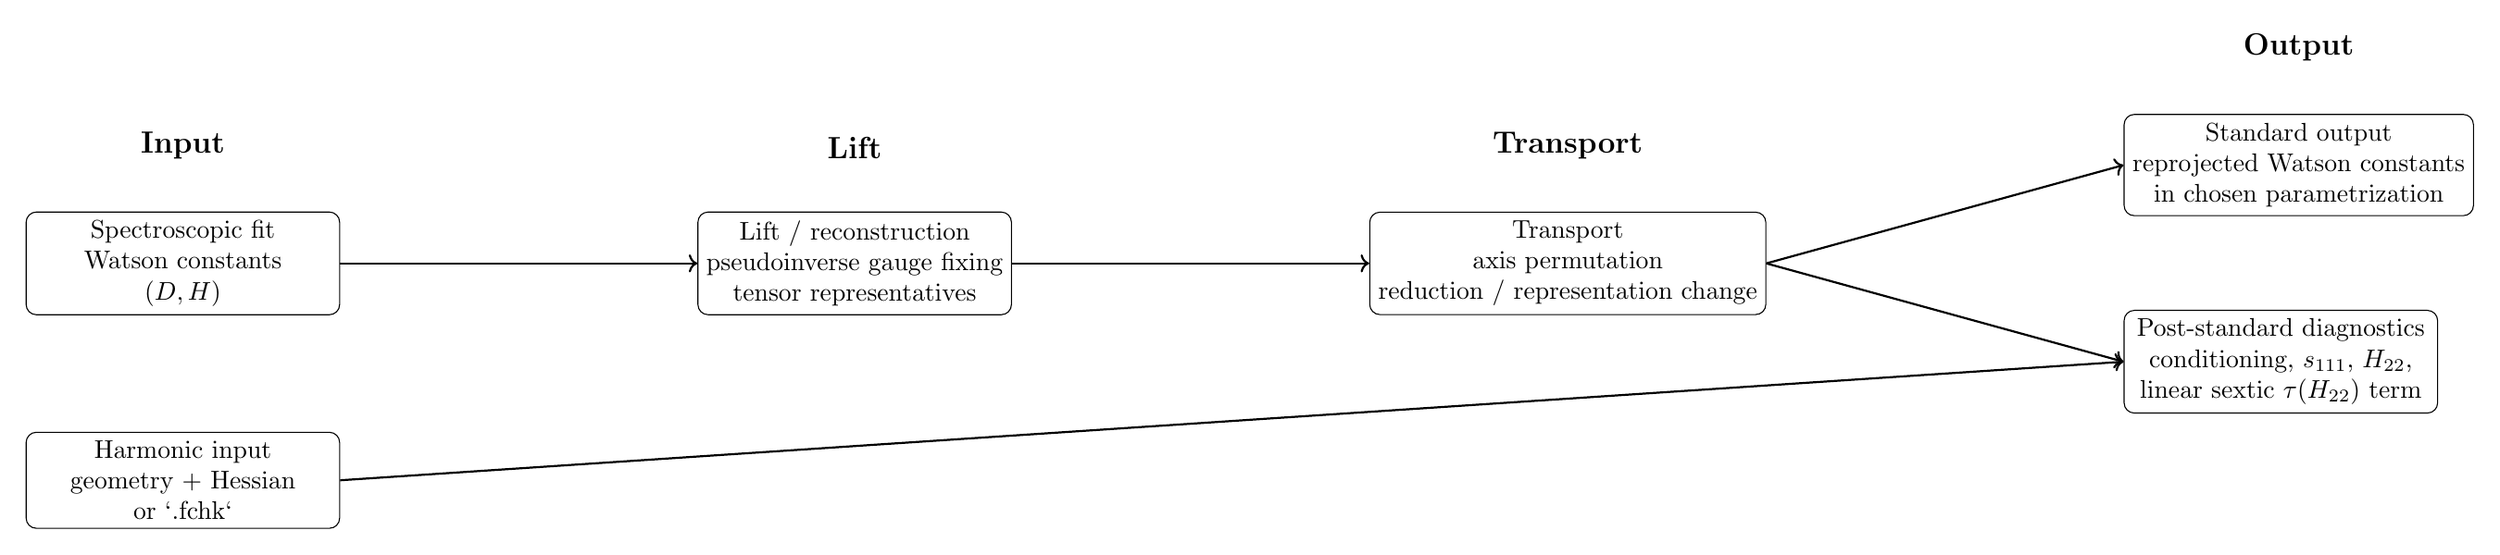
\begin{tikzpicture}[
box/.style={
rectangle,draw,rounded corners,
align=center,
minimum width=4.3cm,
minimum height=1.3cm
},
arrow/.style={->,thick}
]

% INPUTS
\node[box] (fit)
{Spectroscopic fit\\Watson constants\\$(D,H)$};

\node[box,below=1.6cm of fit] (harm)
{Harmonic input\\geometry + Hessian\\or `.fchk`};

\node[above=0.6cm of fit] {\large \textbf{Input}};

% LIFT
\node[box,right=4.9cm of fit] (lift)
{Lift / reconstruction\\pseudoinverse gauge fixing\\tensor representatives};

\node[above=0.6cm of lift] {\large \textbf{Lift}};

% TRANSPORT
\node[box,right=4.9cm of lift] (transport)
{Transport\\axis permutation\\reduction / representation change};

\node[above=0.6cm of transport] {\large \textbf{Transport}};

% OUTPUT
\node[box,right=4.9cm of transport,yshift=1.35cm] (reproj)
{Standard output\\reprojected Watson constants\\in chosen parametrization};

\node[box,right=4.9cm of transport,yshift=-1.35cm] (diag)
{Post-standard diagnostics\\conditioning, $s_{111}$, $H_{22}$,\\linear sextic $\tau(H_{22})$ term};

\node[above=0.6cm of reproj] {\large \textbf{Output}};

% ARROWS
\draw[arrow] (fit.east) -- (lift.west);
\draw[arrow] (harm.east) -- (diag.west);
\draw[arrow] (lift.east) -- (transport.west);
\draw[arrow] (transport.east) -- (reproj.west);
\draw[arrow] (transport.east) -- (diag.west);

\end{tikzpicture}
}

\caption{
Operational structure of the present framework. Standard quartic and sextic
centrifugal distortion constants are lifted from Watson parametrizations to
tensor representatives through pseudoinverse gauge fixing, transported under
representation changes, and reprojected onto the target Hamiltonian
parametrization. Optional harmonic input is only needed for post-standard
diagnostics, namely the quartic $H_{22}$ contribution and its first sextic
linear analogue.
}

\label{fig:ceditt3_scheme}
\end{figure}


The conceptual hierarchy behind this workflow is summarized separately
in Fig.~\ref{fig:ceditt3_hierarchy}. Harmonic geometry first defines
the inertia tensor, the first derivative $\mu_1$ generates the minimal
linear tensor sector shared by standard quartic and standard sextic
centrifugal distortion, and cubic force constants introduce the first
genuinely nonlinear layer.

\begin{figure}[t]
\centering
\resizebox{0.78\textwidth}{!}{
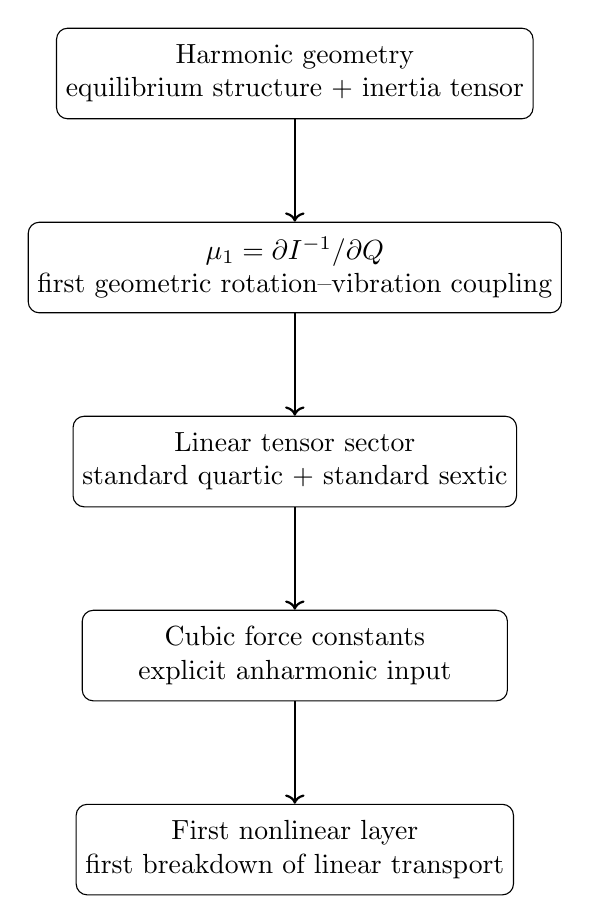
\begin{tikzpicture}[
box/.style={
rectangle,draw,rounded corners,
align=center,
minimum width=5.4cm,
minimum height=1.15cm
},
arrow/.style={->,thick}
]

\node[box] (harm) {Harmonic geometry\\equilibrium structure + inertia tensor};
\node[box,below=1.3cm of harm] (muone) {$\mu_1=\partial I^{-1}/\partial Q$\\first geometric rotation--vibration coupling};
\node[box,below=1.3cm of muone] (linear) {Linear tensor sector\\standard quartic + standard sextic};
\node[box,below=1.3cm of linear] (cubic) {Cubic force constants\\explicit anharmonic input};
\node[box,below=1.3cm of cubic] (nonlinear) {First nonlinear layer\\first breakdown of linear transport};

\draw[arrow] (harm.south) -- (muone.north);
\draw[arrow] (muone.south) -- (linear.north);
\draw[arrow] (linear.south) -- (cubic.north);
\draw[arrow] (cubic.south) -- (nonlinear.north);

\end{tikzpicture}
}

\caption{
Conceptual hierarchy revealed by the tensor formulation. Harmonic
geometry defines the inertia tensor, its first derivative $\mu_1$
generates the minimal linear tensor sector governing standard quartic
and standard sextic centrifugal distortion constants, and cubic force
constants introduce the first genuinely nonlinear layer.
}

\label{fig:ceditt3_hierarchy}
\end{figure}


\subsection{Standard quartic sector}

In the standard quartic sector, the relevant rovibrational content is
generated entirely by the first-level inverse-inertia derivative
$\mu_1$, or, equivalently, by its Coriolis-coupling description. The
standard quartic contribution therefore remains fully inside the
first-level tensorial language.

At the spectroscopic level, the quartic constants are obtained after
projection of the quartic tensor representative onto Watson's operator
basis. At the tensor level, however, the standard quartic problem is
linear: once the representative has been fixed by pseudoinverse
reconstruction, representation changes are implemented by linear
transport of the tensor itself. This is the first half of the
standard linear sector developed in the present work.

\subsection{Standard sextic sector}

The sextic problem is structurally richer, but in its standard form it
still closes on the same first-level tensorial language. The key
result of the present analysis is that the standard sextic geometry
sector does not require second derivatives of the inertia tensor as
primitive objects. Instead, the standard sextic geometry contributions
can be written in terms of the same first-level data that govern the
standard quartic problem, together with Coriolis couplings and the
explicit anharmonic cubic force constants.

This is physically important. If second inertia derivatives were
genuinely primitive already at the level of standard sextics, then
quartics and sextics would not belong to a common linear transport
sector. By showing that the standard sextic geometry sector can be
rewritten without primitive $d^2I/dQ^2$, the present framework
identifies the correct baseline from which genuinely new
post-standard tensorial objects can later be recognized. This is the
second half of the standard linear sector.

In this sense, the ``standard sextic sector'' should be understood
strictly as the sextic content that can still be expressed in terms of
the same first-level tensorial objects governing the quartic problem.
The explicit cubic-force contribution is then precisely the first place
where this minimal linear closure must be enlarged.

\subsection{Unified standard linear sector}

The standard quartic and standard sextic problems therefore admit a
common tensorial description. They are both governed by the same
first-level geometric language, and both are transported between
representations by the same pseudoinverse-lift, tensor-transport, and
reprojection mechanism.

This observation provides a unified tensor interpretation of the
standard quartic and sextic sectors and explains why their
representation dependence can be treated within the same transport
framework.

This motivates the central notion of the present paper: there is a
standard linear sector of centrifugal-distortion theory. In this
sector, fitted Watson constants and
directly computed rovibrational quantities can be compared on the same
tensorial footing, without introducing additional primitive objects
beyond those already present in the standard construction.

The corresponding representation equivalence should be understood precisely at the
level of this minimal linear sector. It is this restricted but
physically important domain, rather than the full higher-order
effective Hamiltonian, that is shown here to admit a common tensorial
transport picture.

In practical quantum-chemical calculations the standard perturbative
sector typically includes only the $H_{12}H_{12}$ contributions. Under
these conditions the linear transport framework remains valid, and the
breakdown discussed here should be interpreted mainly as a formal
limitation of the representation-equivalence structure rather than as a
practical computational difficulty.

\subsection{First breakdown in the quartic sector: \texorpdfstring{$H_{22}$}{H22}}

The first departure from this standard linear sector occurs in the
quartic channel $H_{22}$. This channel is structurally simple enough
to be isolated, yet it already forces the appearance of a genuinely
new tensorial object.

In the present work, the expression ``first breakdown'' has a precise
meaning. It denotes the first contribution to the effective
centrifugal-distortion problem that cannot be represented within the
minimal first-level linear tensor sector generated by $\mu_1$ and its
standard geometric descendants. Operationally, it is therefore the
first term that makes linearly transported Watson parameter sets in
different representations cease to be strictly equivalent descriptions
of the same fitted content.

Physically, $H_{22}$ is the first contribution that depends on the
second response of the inertia tensor to vibrational motion. In the
notation adopted here, the full second inverse-inertia derivative may
be written as
\begin{equation}
\mu_2 = B(\mu_1) - N,
\end{equation}
where $B(\mu_1)$ is the bilinear closure generated algebraically from
the first-level object $\mu_1$, while $N$ is the intrinsic second-level
tensor not reducible to the standard first-level sector.

This decomposition is the physical core of the breakdown. The term
$B(\mu_1)$ does not introduce a new tensorial layer; it is the
algebraic closure of the already known first-level geometry. By
contrast, $N$ represents the genuinely new part of the second-order
inertia response. The quartic channel $H_{22}$ is therefore the first
place where the standard linear language is no longer sufficient by
itself.

In this sense, $H_{22}$ is not merely an additional post-standard
correction. It is the first identifiable tensorial marker of a new
coupling mechanism: the first point at which the effective quartic
Hamiltonian depends on an intrinsic second-level geometric object
rather than only on the closure of the first-level one. This is why
it is used in the present work as the primary diagnostic of the
breakdown of the standard sector. The important point is not that
$H_{22}$ must be the numerically largest post-standard quartic
contribution in every molecule, but that it is the first contribution
expected to break the linear representation transport that governs the
standard quartic and sextic sectors.

This role is specific. Purely vibrational channels such as
$H_{30}H_{30}$ do not introduce a new rotational tensorial level of
the same type, and mixed channels such as $H_{12}H_{30}$ still couple
anharmonicity to the first-level rotational object. For this reason
$H_{22}$ is the natural first candidate for the breakdown of linear
representation equivalence, even if other channels may later become
numerically larger in absolute value.

Whether $H_{22}$ becomes quantitatively important depends on the
molecule. The results section shows that it is small in systems such
as formaldehyde, where the standard perturbative picture is already
rather reliable, and larger in water, where the difference between
standard VPT-based and higher-level results is more pronounced. The
role of $H_{22}$ is therefore diagnostic rather than universal: it
signals the first failure of the standard linear sector, but does not
claim to exhaust the whole beyond-standard correction.

Beyond this point the tensor framework itself does not cease to apply.
What fails is the sufficiency of the minimal first-level linear sector.
Additional tensorial layers must then be introduced, and the simple
representation-equivalent transport picture of the standard sector no
longer closes by itself.

\subsection{First sextic analogue: linear response in \texorpdfstring{$\tau(H_{22})$}{tau(H22)}}

The same logic extends naturally to the sextic side. Within the
standard sextic geometry functional, the quartic tensor enters
explicitly. Therefore, once the standard quartic contribution is
replaced by
\begin{equation}
\tau = \tau_{\mathrm{std}} + \tau(H_{22}),
\end{equation}
the first post-standard sextic contribution is the term linear in
$\tau(H_{22})$.

Here $\tau(H_{22})$ denotes the quartic tensor representative
generated by the $H_{22}$ channel. The corresponding linear-response
term is the natural sextic analogue of the quartic channel $H_{22}$:
it is the first sextic contribution that probes the breakdown of the
standard linear sector while still remaining simple enough to be
treated as a diagnostic rather than as part of a full higher-order
theory.

This point should be read in strict analogy with the quartic case.
The quantity is not introduced as a complete post-standard sextic
correction, but as the first controlled way in which the new quartic
tensorial level feeds into the sextic problem. In that sense it
provides the sextic companion of the quartic $H_{22}$ diagnostic.

At the physical level, the reason cubic anharmonicity becomes the first
source of nonlinearity is that it couples vibrational modes in a way
that can no longer be reduced to the first-level geometric response of
the inverse inertia tensor. Once these cubic couplings enter
explicitly, new tensor combinations appear that do not close within the
minimal linear sector generated by $\mu_1$ and its standard geometric
descendants.

\subsection{Relation to earlier tensorial formulations}

The tensorial structure underlying centrifugal distortion is not new
in itself. It is already implicit in the classical formulations of
Watson and Mills and in later rotational-tensor treatments of
effective Hamiltonians.\cite{Watson1968,Watson1977,Mills1972,Kirschner1983}
What is new here is not the existence of
tensorial content behind Watson constants, but the use of that content
as the explicit operational layer for:
\begin{enumerate}
\item pseudoinverse reconstruction from spectroscopic parameter sets,
\item transport between reductions and principal-axis representations,
\item common treatment of standard quartic and standard sextic sectors,
\item identification of the first post-standard diagnostics.
\end{enumerate}

The present work therefore differs from earlier tensorial viewpoints
less by introducing a new kind of tensor than by making the tensor
representatives the center of the computational and interpretative
workflow. In this sense, the novelty lies in the combination of
tensor reconstruction, gauge fixing, representation transport, and
controlled identification of the first breakdown terms.

\subsection{Scope of the present work}

The present paper is therefore not a theory of the full higher-order VPT problem.
Its scope is deliberately narrower:
\begin{enumerate}
\item identify the standard linear quartic/sextic sector;
\item formulate its transport between representations and reductions for
nondegenerate asymmetric tops;
\item isolate the first quartic and sextic diagnostics of its breakdown.
\end{enumerate}

The detailed tensor derivations, the explicit BCH/contact-transformation
coefficients, the quartic and sextic projection formulas, and the full
construction of the $H_{22}$ and $\tau(H_{22})$ diagnostics are
deferred to the appendices. The exact symmetric-top, spherical-top, and
linear-molecule limits require separate symmetry-adapted projections because
the asymmetric-top Watson formulas become singular or collapse there. In this
sense there is no single continuous parametrization that carries the same
spectroscopic coordinates smoothly across linear molecules, symmetric tops,
spherical tops, and nondegenerate asymmetric tops. The tensorial hierarchy,
however, survives in all cases, and the corresponding case-adapted equations
are given explicitly in a dedicated appendix. Continuity therefore holds at
the tensorial level, not at the level of a single universal set of fitted
spectroscopic constants.


\section{Results and Discussion}

\subsection{From tensor transport to spectroscopic use}

The main value of the present framework is not only conceptual. Once quartic
and sextic centrifugal distortion constants are lifted to their tensor
representatives, the same machinery may be used in practical spectroscopic
workflows to:
\begin{enumerate}
\item compare parameter sets obtained in different reductions or
representations;
\item transport fitted or computed constants from one representation to
another;
\item identify numerically ill-conditioned representation changes before a new
fit is attempted;
\item monitor the first breakdown of the standard linear sector through the
diagnostics $H_{22}$ and, on the sextic side, the term linear in
$\tau(H_{22})$.
\end{enumerate}

This section is therefore organized around real use cases rather than around
formal properties alone. Dimethylsulfoxide is used to illustrate
representation instability within the standard sector. Formaldehyde and
thioformaldehyde illustrate the transport of sextic standard constants through
their canonical tensor content. The hydroxybenzonitrile (HBN) isomers and the uridine molecule shown in Figure \ref{fig:structures} are then used as quartic test beds, large enough to make the practical choice of computational hierarchy relevant. 

\begin{figure*}[t]
\centering

\includegraphics[width=1.0\linewidth]{molecules_CeDiTT.jpg}
\caption{Structures of hydroxybenzonitrile (HBN) isomers and uridine.}
\label{fig:structures}
\end{figure*}

Water and formaldehyde are then
used to show how the quartic diagnostic $H_{22}$ behaves when the standard
VPT2 picture is respectively under stress or still reliable. Taken together,
these examples show that the present framework is not merely a reformulation
of known theory, but a practical tool for spectroscopic analysis. The analyses
discussed below are implemented in the app workflow: the standard quartic and
sextic transport steps start directly from centrifugal distortion constants,
whereas the post-standard diagnostics $H_{22}$ and $\tau(H_{22})$ use
optional harmonic input (`.fchk` or `xyz + Hessian`).

From the validation point of view, the role of these examples is also
well-defined. DMSO validates quartic transport in a case where representation
conditioning is known to be problematic. H$_2$CO and H$_2$CS validate the
standard sextic transport machinery against experimental and variational
parameter sets. H$_2$O versus H$_2$CO validates the first-breakdown diagnostic
$H_{22}$ by showing that it grows precisely where the standard VPT2 picture is
known to be under greater strain. The HBN family finally shows that the same
logic remains meaningful on systems of intermediate size, where computational
hierarchy and transport strategy become practical rather than purely formal
issues.

The quantum-chemical data entering these applications were generated within
the Pisa Composite Scheme (PCS) framework. In particular, two members of the
PCS family play complementary roles. The hybrid PCS2 scheme (HPCS2), based on
the B3LYP/6-31+G* level of theory, provides reliable anharmonic contributions
to rotational spectroscopic parameters. The double-hybrid PCS3 scheme
(DPCS3), based on the revDSD-PBEP86-D3BJ functional combined with the 3F12-
basis set, provides a more accurate harmonic baseline through improved
equilibrium structures and harmonic force fields.\cite{BDPCS3_2023}

This level of accuracy is already spectroscopically meaningful. In the
DPCS3//HPCS2 strategy, supplemented when needed by simple bond-length
corrections as in the BDPCS3 protocol, relative errors on rotational
constants may be pushed to the order of $0.1\%$,\cite{acr_2026} while 
quartic and sextic centrifugal-distortion constants can be described at 
the few-percent level.\cite{Boussessi_quartic,Boussessi_sextic}

Equally important, these calculations are no longer restricted to textbook
benchmarks: workflows of this type are now feasible for molecules with several
tens of atoms, up to the $\sim 50$-atom scale.\cite{hormones_2024,fast_dvib_2025}
This is precisely why the transformation problem addressed here has become
important in practice. Once quartic and sextic constants can be computed with
this level of accuracy on medium-sized systems, a representation analysis is
needed not only for conceptual clarity but also for the practical comparison
between fits, direct calculations, and transported parameter sets.

This distinction matters directly for the present paper. The standard
tensor-transport machinery and the quartic $H_{22}$ diagnostic are anchored in
the harmonic model, whereas the standard sextic anharmonic sector depends on
the cubic force field. For medium-sized molecules this computational hierarchy
is now realistic: modern workflows already provide accurate quadratic force
fields and semi-diagonal cubic force constants on systems far beyond the
traditional small-molecule benchmark set.\cite{cubic-vib_2024,cubic-internal_2024,fast_dvib_2025,hormones_2024,RotBio_2023,AnnRevPC_2023}
In that regime, a low-cost
diagnostic of the limits of standard perturbative transport is especially
useful, because the harmonic information is already affordable and accurate
even when a full post-standard treatment is not.

Operationally, this leads to a natural three-level hierarchy on the sextic
side:
\begin{enumerate}
\item harmonic model only: geometry sector and first H$_{22}$-induced sextic
diagnostic;
\item harmonic model plus semi-diagonal cubic sector: reduced sextic
prediction at nearly linear cost;
\item full cubic field: genuine three-index remainder and complete standard
sextic prediction.
\end{enumerate}
This hierarchy is important for the present paper because it connects the
formal tensor decomposition directly to the computational resources that are
realistically available for medium-sized molecules.

The corresponding practical workflow is therefore straightforward.
Starting from fitted Watson constants alone, one may perform standard
quartic and sextic transport between representations and evaluate the
conditioning diagnostics associated with the lift--transport--reproject
procedure. If harmonic input is also available in the form of geometry
plus Cartesian Hessian (or equivalently an input \texttt{.fchk} file),
one obtains in addition the standard quartic tensor, the quartic
$H_{22}$ diagnostic, the sextic geometry sector, and the first sextic
diagnostic induced by $\tau(H_{22})$. If semi-diagonal cubic data are
added, the reduced sextic prediction becomes available at nearly linear
cost in the number of modes, whereas adding the full cubic field yields
the genuine three-index remainder and thus the complete standard sextic
prediction. In this sense, the present framework does not require a
single all-or-nothing computational protocol, but naturally supports a
hierarchy of inputs, costs, and outputs.

\subsection{DMSO: representation transport and numerical instability}

The choice of Watson reduction and principal-axis representation is known to
affect the numerical stability of centrifugal-distortion fits. This is
particularly clear for dimethylsulfoxide (DMSO), which was analyzed in detail
by Margul\`es \emph{et al.}\cite{Margules2010} and already served as a key case
in the previous version of this work.

DMSO is especially useful here because the rotational constants $A$ and $B$
are close in magnitude. As a consequence, representation changes involving the
$I^r \leftrightarrow III^r$ conversion may become poorly conditioned, even
though the underlying tensor content remains the same. In this situation the
present tensorial strategy is particularly informative. One starts from a
given quartic Watson parameter set, reconstructs the reduced quartic tensor by
pseudoinverse lifting, transports that tensor under the required axis
permutation, and finally reprojects the result onto the target Watson
representation. In the present work, this entire workflow was executed through
the app, exactly in the same form in which it would be used in practical
spectroscopic analysis.

When this is done for DMSO, the individual Watson constants can vary strongly
between representations, especially in the anisotropic sector. This is not a
failure of the tensor algorithm. It is precisely the phenomenon that the
framework is meant to disentangle. The large variation is driven by the
conditioning of the chosen parametrization, not by a change in the underlying
quartic rovibrational content. This is seen most clearly by comparing the
reconstructed reduced quartic tensor $\tau'$ rather than the raw Watson
constants: its spectral invariants remain unchanged, up to the expected
permutation similarity, across representation transport.

The DMSO example therefore plays two roles. First, it validates the tensor
transport procedure on a realistic spectroscopic case for which representation
dependence is known to be severe. Second, it shows why a tensor-level analysis
is operationally preferable to a direct comparison of Watson constants.
Quantities such as $s_{111}$ and the condition number of the transport provide
practical indicators of whether a nominally equivalent representation is
actually a stable one for fitting purposes.

The numerical content of Table~\ref{tab:DMSO_constants} illustrates this point
directly. In the $A$ reduction, the change from $I^r$ to $III^r$ leaves some
constants only moderately affected, but others vary dramatically. The clearest
example is $\delta_K$, which changes from a value of order $1$ kHz in the
$I^r$ representation to a value of order $10$--$50$ kHz in the $III^r$
representation. The corresponding $s_{111}$ values show the same trend: while
they remain very small in the stable representations, they grow sharply in the
ill-conditioned one. In the $S$ reduction the same phenomenon is visible in a
less extreme but still clear form, with the anisotropic constants responding
much more strongly than the isotropic ones to the representation change.

These numerical variations are too large to be interpreted as simple changes
in underlying rovibrational physics. They are instead the signature of a
representation problem: the same physical quartic content is being described
through a parametrization whose conditioning deteriorates when the transformation
denominators become small. This is exactly the kind of situation in which the
tensor formulation is useful, because it separates the physical content from
the instability of the Watson coordinates.

\begin{table*}[t]
\centering
\caption{Quartic centrifugal distortion constants and corresponding
$s_{111}$ parameter for dimethylsulfoxide in different Watson
representations (kHz). Rotational constants used in the analysis are
$A=7036.6$, $B=6910.8$, $C=4218.78$ MHz for the experimental fit and
$A=6749.88$, $B=6716.88$, $C=4052.83$ MHz for the HPCS2 calculation.}

\begin{tabular}{lccccc}
\hline
Constant & $I^r$ (QM) & $I^r$ (fit) & $III^r$ (QM) & $III^r$ (fit) & $III^r$ (fit, transf) \\
\hline

\multicolumn{6}{c}{A reduction} \\

$\Delta_J$    & 3.9912 & 4.0509 & 6.5456 & 6.6268 & 6.6327 \\
$\Delta_{JK}$ & -4.4009 & -4.4528 & -12.0641 & -12.1574 & -12.1981 \\
$\Delta_K$    & 6.3961 & 6.7065 & 6.3961 & 6.6726 & 6.7065 \\
$\delta_J$    & 1.5568 & 1.4549 & -0.2796 & -0.1648 & -0.1640 \\
$\delta_K$    & 1.1788 & 1.2856 & -29.5443 & -46.8755 & -29.7583 \\
$s_{111}$     & $5.6\times10^{-6}$ & $5.3\times10^{-7}$ & $-4.86\times10^{-4}$ & $-1.3\times10^{-6}$ & $-1.73\times10^{-3}$ \\

\hline

\multicolumn{6}{c}{S reduction} \\

$D_J$         & 4.5954 & 3.4631 & 6.2204 & 6.0892 & 6.6843 \\
$D_{JK}$      & -8.0260 & 0.9259 & -12.9010 & -8.9372 & -8.7376 \\
$D_K$         & 9.4171 & 3.7676 & 9.4171 & 3.9893 & 3.7676 \\
$d_1$         & 1.5568 & 1.4549 & -0.0507 & 0.1641 & 1.5850 \\
$d_2$         & 0.3021 & 0.2939 & -0.1832 & -0.2717 & -0.1126 \\
$s_{111}$     & $7.8\times10^{-8}$ & $7.5\times10^{-8}$ & $3.6\times10^{-8}$ & $3.5\times10^{-8}$ & $3.5\times10^{-8}$ \\

\hline
\end{tabular}

\label{tab:DMSO_constants}
\end{table*}

The same conclusion is seen more clearly at the tensor level. While the Watson
constants vary strongly, the spectral content of the reconstructed quartic
tensor is stable under representation transport. This is illustrated in
Table~\ref{tab:DMSO_tauprime}, where the eigenvalues and polynomial invariants
of the reduced quartic tensor are reported for the fitted and transported DMSO
parameter sets. The transported $III^r$ row reproduces the $I^r$ tensor
invariants within numerical precision, as expected for a single underlying
quartic tensor seen in different representations.


\begin{table*}[t]
\centering
\caption{Spectral invariants of the reduced quartic tensor $\tau'$ for
dimethylsulfoxide obtained from different Watson representations. The
$III^r$ (fit, transf) row corresponds to the tensor obtained by transporting
the $I^r$ fit through the tensor algorithm. Equality of the eigenvalues and
invariants demonstrates the representation independence of the tensor
description. Small deviations in the independently fitted $III^r$ row arise
from rounding of the published spectroscopic constants.}

\begin{tabular}{lcccccc}
\hline
Representation & $\lambda_1$ & $\lambda_2$ & $\lambda_3$ & $I_1^{(\tau')}$ & $I_2^{(\tau')}$ & $I_3^{(\tau')}$ \\
\hline
$I^r$ (fit)           & -2.4752 & -8.7629 & -46.3875 & -57.6256 & 542.9974 & -1006.1386 \\
$III^r$ (fit)         & -2.4849 & -8.6332 & -46.4642 & -57.5824 & 538.0495 & -996.7901 \\
$III^r$ (fit, transf) & -2.4752 & -8.7629 & -46.3875 & -57.6256 & 542.9974 & -1006.1386 \\
\hline
\end{tabular}

\label{tab:DMSO_tauprime}
\end{table*}


The numerical pattern in Table~\ref{tab:DMSO_tauprime} is the key counterpoint
to Table~\ref{tab:DMSO_constants}. The transported $III^r$ row reproduces the
$I^r$ eigenvalues and invariants essentially exactly, confirming that the
tensor algorithm preserves the intrinsic quartic content under representation
change. By contrast, the independently fitted $III^r$ row shows only small
deviations, entirely consistent with the finite precision and rounding of the
published constants. The important point is therefore not that the Watson
constants look different, but that the reconstructed tensor remains the same
within the expected numerical accuracy. This is the operational meaning of
representation-equivalent transport in a real spectroscopic case.

\subsection{Standard sextics as transported tensor content}

The sextic side of the theory is illustrated most cleanly by small asymmetric
tops for which complete sextic parameter sets are available from both
experiment and variational calculations. Formaldehyde and thioformaldehyde are
natural examples because Ref.~\citenum{Dinu2022} reports sextic constants in
Watson's $S$ reduction and $I^r$ representation for both molecules.

In the present framework these sextic constants are not treated as seven
independent spectroscopic coordinates. Instead, they are decomposed as
\begin{equation}
\mathbf H_S = \mathbf B_{I^r}\,\boldsymbol\sigma + \mathbf r,
\end{equation}
where $\boldsymbol\sigma$ contains the five physical sextic coordinates of the
canonical sector and $\mathbf r$ is the residual in the complementary
two-dimensional space. The vector $\boldsymbol\sigma$ is the transported
physical content, whereas $\mathbf r$ acts as a diagnostic of how closely the
input parameter set follows the modeled standard sextic subspace.

For H$_2$CO and H$_2$CS, the canonical coordinates obtained from experiment and
from the VCI/PFIT parameter sets are very similar. This is exactly the type of
behaviour one wants from a transported tensor representative: even when the
individual Watson constants differ, the physical content extracted from them
remains stable. The residual norms are not exactly zero, but this is expected
for finite-precision spectroscopic parameter sets and should not be read as a
failure of the method. Rather, the residual provides a compact measure of the
distance between a real fitted parameter set and the idealized standard sextic
subspace used in the tensor model.

This example is important for the main thesis of the paper. It shows in a real
spectroscopic setting that the standard sextic sector can be handled by the
same lift--transport--reprojection logic as the quartic one, even though its
effective-Hamiltonian parametrization is richer. In other words, the sextic
problem does not require a distinct transport philosophy. It still belongs to
the same standard linear sector.

At the same time, the sextic side of the present work is not merely a
transport exercise. The equations are written explicitly in terms of the
geometric quantities $c_1$, $c_2$, and $\tau$, plus a separate cubic-force
contribution. This makes it possible, at least in principle, to decompose the
standard sextic sector into geometry, semi-diagonal cubic terms, and the
genuinely three-index cubic remainder. That separation is especially relevant
for medium-sized molecules, where semi-diagonal and full cubic data may be
available at different levels of theory.

The numbers support this conclusion directly. For H$_2$CO, the experimental
and VCI/PFIT values of the canonical coordinates differ only slightly across
all five components: for example, $\sigma_3$ changes from about $3.26$ to
$3.36$ kHz and $\sigma_5$ from about $2.49$ to $2.56$ kHz. For H$_2$CS the
same pattern is seen on a larger absolute scale, with $\sigma_3$ near
$4.81$--$4.86$ kHz and $\sigma_5$ near $3.67$--$3.71$ kHz. Thus the tensor
coordinates retain the chemically expected trend, namely a systematically
larger sextic distortion for the sulfur analogue, while remaining stable under
the experiment/VCI comparison.

Operationally, this sextic decomposition and transport were again obtained
with the app, showing that the same tool handles both quartic and sextic
standard sectors in a uniform way.

The residual norms carry complementary information. They are small enough to
confirm that the published sextic constants lie close to the modeled standard
subspace, but not so small as to suggest an exact algebraic identity at the
level of rounded spectroscopic parameters. This is precisely the regime in
which the residual becomes a useful spectroscopic diagnostic rather than a
formal remainder with no interpretative value.

\subsection{HBN isomers: a medium-sized quartic test bed}

The present framework is not intended only for traditional benchmark
molecules. A useful intermediate test bed is provided by the HBN isomer
family, where accurate quartic constants, representation transforms, and
high-level PCS calculations are all available while the size of the systems is
already representative of modern rotational spectroscopy on medium-sized
molecules.

For the four HBN isomers (\emph{o}-HBN, \emph{p}-HBN, \emph{cis}-m-HBN, and
\emph{trans}-m-HBN), Table~\ref{table:hbn_main} collects the ground-state
rotational constants and quartic centrifugal distortion constants in the
$I^r$ representation and $A$ reduction, together with the transformed
constants in $III^r$ ($A$ reduction) and $I^r$ ($S$ reduction). The same table
also reports the gauge diagnostic $\log_{10}|s_{111}|$. These are exactly the
quantities that a working spectroscopist would want to inspect before deciding
whether a representation change is harmless, numerically delicate, or better
avoided altogether.

The numerical pattern is instructive. In the native $I^r$ ($A$) description,
the quartic constants are small and chemically well behaved across the four
isomers, and the corresponding $\log_{10}|s_{111}|$ values remain in the
$-10$ to $-11$ range. This is the fingerprint of a standard sector that is
still well conditioned. After transport to $III^r$ ($A$), however, the
anisotropic constants become much larger and the magnitude of $s_{111}$ grows
by roughly one to two orders, especially for the more asymmetric members of
the family. This reproduces, on a chemically broader series, the same lesson
already seen for DMSO: what changes strongly under representation transport is
the Watson parametrization, not necessarily the underlying quartic tensor.

The HBN family is especially useful because it bridges the gap between the
classical small-molecule benchmarks and the medium-sized systems that motivate
the present paper. The PCS calculations used here are representative of the
quality of data that is becoming available today for molecules with several
tens of atoms. In this regime, the tensor transport itself is already directly
useful, while the same systems also provide a realistic platform for testing
how far the sextic hierarchy can be pushed with harmonic input, semi-diagonal
cubic data, and eventually the genuine three-index cubic remainder.

\begin{table*}[t]
\centering
\scriptsize
\setlength{\tabcolsep}{4pt}

\caption{Ground-state rotational constants (MHz) and quartic centrifugal
distortion constants (kHz) for the four HBN isomers in the $I^r$
representation (A reduction). Ground-state constants were obtained by
subtracting the HPCS2 vibrational corrections from the equilibrium values
computed at different levels. The diagnostic parameter $s_{111}$ is reported
as $\log_{10}|s_{111}|$. The table further includes quartic constants
transported to $III^r$ (A reduction) and to $I^r$ (S reduction) through the
tensor-transform workflow implemented in the app.}

\begin{tabular}{lccc ccc ccc ccc}
\toprule
& \multicolumn{3}{c}{\textbf{cis-$o$-HBN}}
& \multicolumn{3}{c}{\textbf{$p$-HBN}}
& \multicolumn{3}{c}{\textbf{cis-$m$-HBN}}
& \multicolumn{3}{c}{\textbf{trans-$m$-HBN}} \\
\cmidrule(lr){2-4}
\cmidrule(lr){5-7}
\cmidrule(lr){8-10}
\cmidrule(lr){11-13}
Parameter
& Exp. & HPCS2 & DPCS3
& Exp. & HPCS2 & DPCS3
& Exp. & HPCS2 & DPCS3
& Exp. & HPCS2 & DPCS3 \\
\midrule
\multicolumn{13}{c}{\textbf{Rotational constants (MHz)}} \\
$B_a$ & 3053.7 & 3037.2 & 3062.1 & 5613.0 & 5596.5 & 5638.8 & 3408.9 & 3398.4 & 3418.6 & 3403.1 & 3390.4 & 3412.8 \\
$B_b$ & 1511.3 & 1506.4 & 1512.6 & 990.5 & 986.5 & 990.7 & 1205.8 & 1201.0 & 1206.6 & 1208.5 & 1204.1 & 1209.2 \\
$B_c$ & 1010.8 & 1006.8 & 1012.3 & 841.9 & 838.7 & 842.7 & 890.7 & 887.3 & 891.8 & 891.8 & 888.4 & 892.9 \\
\midrule
\multicolumn{13}{c}{\textbf{Quartic constants in $I^r$ (A reduction) (kHz)}} \\
$\Delta_J$ & 0.038 & 0.0368 & 0.0370 & 0.020 & 0.015 & 0.016 & 0.041 & 0.0387 & 0.0390 & 0.040 & 0.0380 & 0.0383 \\
$\Delta_{JK}$ & 0.624 & 0.619 & 0.6204 & 0.231 & 0.221 & 0.223 & 0.027 & 0.0246 & 0.0250 & 0.020 & 0.0352 & 0.0356 \\
$\Delta_K$ & -0.100 & 0.381 & 0.384 & 9 & 0.918 & 0.922 & 1.180 & 1.173 & 1.1778 & 1.130 & 1.158 & 1.161 \\
$\delta_J$ & 0.011 & 0.010 & 0.010 & 0.005 & 0.003 & 0.003 & 0.014 & 0.014 & 0.014 & 0.014 & 0.014 & 0.014 \\
$\delta_K$ & 0.280 & 0.332 & 0.335 & 0.400 & 0.182 & 0.184 & 0.160 & 0.182 & 0.185 & 0.220 & 0.182 & 0.185 \\
$\log_{10}|s_{111}|$ & -10.43 & -10.33 & -10.33 & -11.27 & -11.71 & -11.71 & -11.36 & -11.20 & -11.19 & -11.00 & -11.19 & -11.18 \\
\midrule
\multicolumn{13}{c}{\textbf{$III^r$ (A reduction)}} \\
$\Delta_J$ & 0.5310 & 0.6411 & 0.6445 & 1.9072 & 0.4028 & 0.4068 & 0.3718 & 0.3818 & 0.3851 & 0.3990 & 0.3839 & 0.3869 \\
$\Delta_{JK}$ & -0.9650 & -1.2412 & -1.2499 & -4.0638 & -0.8502 & -0.8572 & -0.8222 & -0.8700 & -0.8788 & -0.9420 & -0.8703 & -0.8785 \\
$\Delta_K$ & 0.4500 & 0.6168 & 0.6223 & 2.1667 & 0.4563 & 0.4603 & 0.4633 & 0.4988 & 0.5046 & 0.5550 & 0.4963 & 0.5018 \\
$\delta_J$ & 0.1255 & 0.2450 & 0.2461 & 2.3052 & 0.2832 & 0.2847 & 0.2947 & 0.2924 & 0.2937 & 0.2805 & 0.2913 & 0.2921 \\
$\delta_K$ & 0.1150 & 0.2613 & 0.2635 & 2.4500 & 0.3205 & 0.3225 & 0.3750 & 0.3843 & 0.3870 & 0.3925 & 0.3805 & 0.3828 \\
\midrule
\multicolumn{13}{c}{\textbf{$I^r$ (S reduction)}} \\
$D_J$ & 0.0380 & 0.0368 & 0.0370 & 0.0200 & 0.0150 & 0.0160 & 0.0410 & 0.0387 & 0.0390 & 0.0400 & 0.0380 & 0.0383 \\
$D_{JK}$ & 0.6240 & 0.6190 & 0.6204 & 0.2310 & 0.2210 & 0.2230 & 0.0270 & 0.0246 & 0.0250 & 0.0200 & 0.0352 & 0.0356 \\
$D_K$ & -0.1000 & 0.3810 & 0.3840 & 9.0000 & 0.9180 & 0.9220 & 1.1800 & 1.1730 & 1.1778 & 1.1300 & 1.1580 & 1.1610 \\
$d_1$ & 0.5820 & 0.6840 & 0.6900 & 0.8100 & 0.3700 & 0.3740 & 0.3480 & 0.3920 & 0.3980 & 0.4680 & 0.3920 & 0.3980 \\
$d_2$ & -0.5600 & -0.6640 & -0.6700 & -0.8000 & -0.3640 & -0.3680 & -0.3200 & -0.3640 & -0.3700 & -0.4400 & -0.3640 & -0.3700 \\
\bottomrule
\end{tabular}

\label{table:hbn_main}
\end{table*}

The tensor perspective becomes clearer when one moves from transported Watson
constants to the representation-invariant content of the reconstructed quartic
tensor. Table~\ref{table:hbn_tauprime} reports the eigenvalues and polynomial
invariants of $\tau'$ for the HPCS2 HBN series. The two meta isomers are
especially informative: although their transported Watson constants differ
noticeably representation by representation, the tensor invariants show that
their intrinsic quartic content is in fact very similar. This is precisely
the kind of chemically meaningful comparison that is obscured at the level of
the raw Watson coordinates and recovered by the tensor lift.

\begin{table*}[t]
\centering
\caption{Spectral invariants of the reduced quartic tensor $\tau'$ for the
HBN isomers reconstructed from the HPCS2 quartic constants.}

\begin{tabular}{lcccccc}
\toprule
Isomer & $\lambda_1$ & $\lambda_2$ & $\lambda_3$ & $I_1^{(\tau')}$ & $I_2^{(\tau')}$ & $I_3^{(\tau')}$ \\
\midrule
cis-$o$-HBN   & 0.9585 & -0.2946 & -5.1055 & -4.4416 & -3.6721 & 1.4417 \\
$p$-HBN       & 0.0267 & -0.0328 & -4.7299 & -4.7360 & 0.0280 & 0.0042 \\
cis-$m$-HBN   & -0.0243 & -0.2578 & -4.9727 & -5.2548 & 1.4090 & -0.0311 \\
trans-$m$-HBN & -0.0214 & -0.2508 & -4.9566 & -5.2288 & 1.3546 & -0.0266 \\
\bottomrule
\end{tabular}

\label{table:hbn_tauprime}
\end{table*}

For the present paper, the importance of the HBN example is twofold. First, it
shows that the tensor transport machinery remains operational on molecules
that are no longer merely textbook benchmarks. Second, it makes the practical
motivation of the sextic reformulation more concrete: these are exactly the
systems for which the separation between harmonic, semi-diagonal cubic, and
genuine three-index cubic contributions becomes both scientifically useful and
computationally meaningful.

\subsection{Uridine: a demanding dual-level spectroscopic case}

The same framework can be pushed well beyond the medium-sized benchmark level.
Gas-phase uridine provides a demanding example because it combines a
29-atom molecular structure, high-resolution experimental data, and a
computational setting in which a dual-level treatment is both realistic and
informative.\cite{uridine_2015} In the present case, equilibrium rotational
constants are available at the DPCS3 and BDPCS3 levels, while vibrational
corrections and centrifugal distortion constants were obtained at the HPCS2
level. This makes uridine a natural example of the kind of practical
equilibrium-plus-correction strategy that motivates the present tensor
formulation.

In current spectroscopic work on large molecules, HPCS2-quality predictions of
rotational and centrifugal-distortion constants are already a realistic
standard. The present application goes one step further by combining the
improved BDPCS3 equilibrium structure with HPCS2 vibrational corrections,
which we denote as `BDPCS3//HPCS2`. This level of theory is still feasible on
workstations of the kind now routinely used for systems in the
30--50 atom range, but it yields rotational constants with an accuracy that is
already comparable to what much more demanding methods provide for smaller
molecules. On this basis, a meaningful analysis of centrifugal distortion
constants also becomes possible.

Table~\ref{tab:uridine_rotational_duallevel} compares the experimental
ground-state rotational constants with the theoretical `HPCS2//HPCS2`,
`DPCS3//HPCS2`, and `BDPCS3//HPCS2` values. The HPCS2 vibrational corrections
are clearly not negligible, especially for the largest rotational constant,
and their inclusion is essential for any meaningful comparison with
experiment. The dual-level comparison is also selective: the
`BDPCS3//HPCS2` combination gives the best agreement with the observed
ground-state constants, reaching a mean absolute percentage error of about
$0.20\%$, compared with about $0.44\%$ for `HPCS2//HPCS2` and about
$0.53\%$ for `DPCS3//HPCS2`. This is already a quantitatively significant
result for a 29-atom system.

\begin{table*}[t]
\centering
\scriptsize
\caption{Uridine as a demanding dual-level case. Experimental ground-state
rotational constants are from Ref.~\citenum{uridine_2015}. The notations
`HPCS2//HPCS2`, `DPCS3//HPCS2`, and `BDPCS3//HPCS2` indicate that the
equilibrium constants are taken at the first level of theory and corrected by
HPCS2 vibrational contributions. The last row reports the mean absolute
percentage error (MAE\%) with respect to experiment.}

\begin{tabular}{lcccc}
\hline
Constant & Exp. ($B_0$) & HPCS2//HPCS2 & DPCS3//HPCS2 & BDPCS3//HPCS2 \\
\hline
$A$ (MHz) & 885.98961(14) & 881.93503 & 880.81087 & 883.90684 \\
$B$ (MHz) & 335.59622(35) & 334.44150 & 334.13848 & 335.10385 \\
$C$ (MHz) & 270.11210(20) & 268.70421 & 268.76154 & 269.53137 \\
\hline
MAE (\%) & --- & 0.441 & 0.531 & 0.199 \\
\hline
\end{tabular}
\label{tab:uridine_rotational_duallevel}
\end{table*}

The quartic constants are equally informative. The supplied geometry is
already in the $I^r$ representation, so the HPCS2 quartic constants can be
transported directly to alternative representations through the tensor
workflow. Table~\ref{tab:uridine_quartic_comparison} reports the native $I^r$
and transported $III^r$ values. Only one quartic constant, $D_J$, was
resolved experimentally, with a value of $0.0115(10)$ kHz. The native $I^r$
prediction, $D_J = 0.00873$ kHz, lies in the same range, whereas the
transported $III^r$ set shows a much stronger reshuffling of the anisotropic
quartic content.

This point is spectroscopically useful. For a molecule of this size a full
quartic fit is difficult, and the experiment could resolve only one quartic
parameter. The calculated constants, however, indicate that at least three
quartic terms are likely to be spectroscopically relevant: besides $D_J$, the
native $I^r$ values of $D_{JK}$ and $D_K$ are also appreciable on the scale
of the fit. In this sense the tensor-transported theoretical quartics can
guide the construction of an experimentally stable Hamiltonian by indicating
which additional distortion terms are worth introducing before the fit becomes
overparameterized. The same calculations also indicate that the sextic
constants are far too small to be expected in the present experiment, so the
quartic sector remains the relevant target for any improved fit.

\begin{table*}[t]
\centering
\scriptsize
\caption{Uridine quartic centrifugal distortion constants from the HPCS2
vibrational treatment, reported in the native $I^r$ representation and after
transport to $III^r$. The supplied geometry is already in the $I^r$
representation. Only $D_J$ was resolved experimentally.}

\begin{tabular}{lccc}
\hline
Quantity & Experiment & HPCS2 ($I^r$) & HPCS2 ($III^r$) \\
\hline
$\Delta_J$ (kHz) & --- & 0.010458 & 0.034881 \\
$\Delta_{JK}$ (kHz) & --- & 0.147760 & 0.074491 \\
$\Delta_K$ (kHz) & --- & -0.097394 & -0.097394 \\
$\delta_J$ (kHz) & --- & 0.000760 & -0.012972 \\
$\delta_K$ (kHz) & --- & 0.061064 & -0.050023 \\
\hline
$D_J$ (kHz) & 0.0115(10) & 0.008729 & 0.066718 \\
$D_{JK}$ (kHz) & --- & 0.158135 & -0.116532 \\
$D_K$ (kHz) & --- & -0.106040 & 0.061792 \\
$d_1$ (kHz) & --- & -0.000760 & 0.012972 \\
$d_2$ (kHz) & --- & -0.000865 & 0.015919 \\
\hline
\end{tabular}
\label{tab:uridine_quartic_comparison}
\end{table*}

The contrast between representations and reductions is already visible at the
level of Table~\ref{tab:uridine_quartic_comparison}. In the native $I^r$
representation the symmetrically reduced constants identify a relatively clear
hierarchy, with $D_J$, $D_{JK}$, and $D_K$ standing out as the only quartic
terms of potentially observable size. After transport to $III^r$, by
contrast, the anisotropic quartic content is redistributed much more strongly:
the $A$- and $S$-reduced constants remain mathematically equivalent, but they
no longer provide the same intuitive or numerically stable basis for fitting.
This is precisely the type of situation in which tensor transport becomes
useful. A fit based on a single quartic constant can reproduce the data, but
it need not return the parameter that would be obtained in a more complete
representation-aware treatment. The comparison with theory therefore suggests
that a constrained fit, with the additional quartic terms introduced together
with physically motivated uncertainty bounds, would be more robust than a fit
in which the whole quartic sector is effectively collapsed onto a single
observed parameter.

Uridine therefore strengthens one of the practical conclusions of the present
paper. For small systems one may aim at benchmark-level predictions of all
spectroscopic constants. For larger systems, the more realistic target is a
selective but physically informed prediction. The present tensor framework is
already useful in that demanding regime: it supports accurate dual-level
rotational constants, transport of quartic constants between representations,
and a theory-guided indication of which distortion terms are worth trying in
an experimental fit.

\subsection{The quartic diagnostic H22}

The standard linear sector is not the whole story, and the key question is how
to detect its first failure in a form that remains simple enough to be
practically useful. This is the role assigned here to the quartic channel
$H_{22}$.

Water and formaldehyde provide a particularly instructive comparison. In
water, the differences between standard VPT-based quartic constants and
higher-level variational results are known to be substantial. In
formaldehyde, the same discrepancies are much smaller. The present diagnostic
follows that trend.

For H$_2$O, the projected quartic contribution generated by $H_{22}$ is
clearly non-negligible on the scale of the fitted quartic constants and of the
VPT/VCI differences, although it is not by itself sufficient to explain the
largest discrepancies. For H$_2$CO, the same diagnostic is dramatically
smaller, by roughly two orders of magnitude. This is exactly the behaviour
expected from a useful first-breakdown indicator: it grows where the standard
picture is under strain and remains small where the standard picture is
already adequate.

The point is not that $H_{22}$ provides the whole correction beyond the
standard quartic sector. The point is that it is the first genuinely new
tensorial contribution, it is simple enough to isolate explicitly, and it can
be computed from the same basic rovibrational information already needed for
the standard problem. In this sense $H_{22}$ is not only a theoretical
channel; it is an operational diagnostic of when one should stop trusting the
standard linear transport picture as quantitatively sufficient. The key issue
is not that $H_{22}$ must be the largest post-standard quartic contribution in
absolute value, but that it is the first term expected to break the linear
equivalence of Watson parameter sets across representations. In this sense two
fits in different representations remain physically equivalent within the
present framework only as long as the $H_{22}$ diagnostic is negligible.

This comparison is important also from the software point of view: $H_{22}$ is
not introduced here as an external post-processing quantity, but as a
diagnostic computed within the same app workflow used for the standard tensor
transport once harmonic input is supplied.

The numerical comparison is most informative in relative rather than absolute
terms. For H$_2$O, the projected $H_{22}$ contributions correspond to
fractions at the $10^{-3}$--$10^{-1}$ level of the fitted quartic constants,
depending on the Watson parameter considered, and they are of the same order
as the smaller VCI--VPT differences even though they do not saturate the
largest ones. For H$_2$CO, the same diagnostic becomes smaller by about two
orders of magnitude and correspondingly negligible as a fraction of the
quartic constants. This relative collapse is the important point: it shows
that the first breakdown of linear transport is much less relevant in the
molecule for which the standard VPT2 picture is already known to be more
reliable.

\subsection{First sextic analogue: linear response in \texorpdfstring{$\tau(H_{22})$}{tau(H22)}}

The same idea extends naturally to the sextic side. Once the standard sextic
geometry functional is written in terms of the standard quartic tensor, the
first post-standard sextic contribution is obtained by replacing the latter by
\begin{equation}
\tau = \tau_{\mathrm{std}} + \tau(H_{22})
\end{equation}
and extracting the term linear in $\tau(H_{22})$.

For H$_2$O this sextic diagnostic is nonzero and measurable, with its largest
component at the level of about $10^3$ Hz. This is much smaller than the
dominant standard sextic constants, so it is not a candidate for a full
post-standard sextic theory by itself. But that is not the point. The
quantity is useful precisely because it is simple, low-cost, and sensitive to
the first way in which the new quartic tensorial level propagates into the
sextic problem.

The natural expectation is that this quantity should remain smaller in systems
for which standard VPT-based and higher-level results are already close, just
as the quartic $H_{22}$ diagnostic does for H$_2$CO. The full H$_2$CO sextic
numerical test requires the corresponding cubic data and may therefore be
added later without changing the logic of the present paper. At the current
stage, the role of the sextic analogue is already clear: it is the first
diagnostic of how the quartic breakdown feeds into the sextic geometry sector.

As for the quartic case, this quantity is available directly in the app
workflow once harmonic input is supplied, so that standard transports and
first-breakdown diagnostics can be inspected within a single operational
environment.

Here again the numerical scale matters. For water the largest component of the
linear sextic response is about $1.3\times 10^3$ Hz, with the dominant effect
appearing in the $\Phi_{aaa}$ channel. Relative to the dominant standard
sextic constants, this corresponds to a correction at about the $10^{-3}$
level: still perturbatively small, but clearly above numerical noise and
therefore defining a genuine post-standard scale. The quantity is therefore
well placed to act as a first warning sign of how the quartic breakdown feeds
into the sextic geometry sector.

\subsection{Scalability and modern spectroscopic scope}

One further point deserves to be stressed. The present framework is not only
suited to small benchmark molecules. Modern rotational spectroscopy and modern
quantum-chemical workflows now routinely reach systems with several tens of
atoms, including flexible organic molecules and biologically relevant species.
The tensor-lifting and transport logic developed here is entirely compatible
with that scale.

This matters for the positioning of the paper. If the framework were useful
only for small benchmark systems, it would remain largely methodological. In
fact, its intended use is broader: the same machinery can organize fitted and
computed centrifugal-distortion constants for medium-sized and large
molecules, help choose numerically stable reductions and representations
before refitting, and signal when the standard linear sector is beginning to
fail even in systems that are far beyond the traditional benchmark set.

This point is reinforced by the current state of practical rovibrational
workflows. Accurate quadratic force fields and semi-diagonal or partial cubic
force information are now becoming available also for medium-sized molecules,
and these data already support high-quality vibrational corrections to the
rotational constants. In that regime, a low-cost indicator of the limits of
the standard perturbative transport picture is particularly valuable. The
quartic $H_{22}$ diagnostic is exactly of this kind, because it is available
from the harmonic model alone, without requiring a full post-standard higher-order VPT
treatment.

The same logic suggests a computationally adapted reading of the sextic
problem. The geometric sextic sector and the first sextic post-standard
diagnostic are already accessible from the harmonic model, while the explicit
cubic contribution may be further decomposed into a semi-diagonal part and a
genuinely three-index remainder. If the latter proves to be small in practice,
then a realistic hierarchy emerges for medium-sized systems: the standard
transport machinery, the quartic $H_{22}$ warning signal, and at least part of
the sextic structure may all be explored before a fully converged high-level
anharmonic treatment becomes affordable.

For water this hierarchy can already be tested explicitly. In the present
benchmark the genuinely three-index cubic remainder vanishes for all ten
standard sextic components, so that the full sextic constants are recovered
exactly from the geometry sector plus the semi-diagonal cubic contribution.
For the dominant $\Phi_{aaa}$ constant, for example, the geometry term is
about $7.72\times 10^5$ Hz and the semi-diagonal cubic contribution about
$9.08\times 10^4$ Hz, yielding the full value of about $8.62\times 10^5$ Hz
with no additional three-index correction. In this sense H$_2$O provides a
clean proof of principle for the computational hierarchy proposed here.

Formaldehyde provides a complementary and more realistic case. Here the
genuinely three-index cubic remainder is no longer zero, but it remains
subleading for the largest sextic constants. For the dominant
$\Phi_{aaa}$ contribution, for instance, the geometry term is about
$4.11\times 10^3$ Hz, the semi-diagonal cubic correction about
$-5.58\times 10^2$ Hz, and the genuine three-index remainder about
$1.18\times 10^2$ Hz, yielding a full value of about $3.67\times 10^3$ Hz.
The three-index part therefore amounts to only about $3\%$ of the total in
the leading channel, even though its relative effect becomes larger for
smaller components. Taken together, H$_2$O and H$_2$CO show that the
semi-diagonal cubic sector can already capture the dominant sextic structure,
while the genuinely three-index part acts as a systematic refinement rather
than as a qualitatively separate contribution.

The same trend persists for thioformaldehyde. For H$_2$CS the dominant
$\Phi_{aaa}$ contribution is about $5.05\times 10^3$ Hz at the geometric
level, with a semi-diagonal cubic correction of about $-3.76\times 10^1$ Hz
and a genuinely three-index remainder of only about $3.3$ Hz, corresponding
to less than $0.1\%$ of the total. Table~\ref{tab:sextic_cubic_hierarchy}
summarizes the dominant sextic component for H$_2$O, H$_2$CO, H$_2$CS, and
F$_2$CO, all reported after transport to a common $I^r$ representation.
F$_2$CO is especially informative because the genuinely three-index cubic
remainder is again very small in the leading channel, amounting to only about
$0.26\%$ of the total. Taken together, these examples suggest that the
genuinely three-index cubic sector is not universally negligible, but often
remains much smaller than the geometry term and the semi-diagonal cubic
contribution in the leading sextic channels. The calculations reported here
were all performed at the HPCS2 level; the purpose is therefore not a
benchmark-quality quantitative assessment of absolute sextic constants, but
the identification of robust trends in the hierarchy of geometric,
semi-diagonal cubic, and three-index cubic contributions.

\begin{table*}[t]
\centering
\caption{Dominant sextic component and decomposition into geometry,
semi-diagonal cubic, and genuine three-index cubic contributions for four
illustrative molecules, all expressed in a common $I^r$ representation. All
values are in Hz. The calculations were performed at the HPCS2 level and are
intended to illustrate trends in the sextic hierarchy rather than
benchmark-quality absolute predictions.}

\begin{tabular}{lcccccc}
\hline
Molecule & Dominant component & Geometry & Cubic 2-index & Cubic 3-index & Total & 3-index / total \\
\hline
H$_2$O  & $\Phi_{aaa}$ & $7.72\times 10^5$ & $9.08\times 10^4$ & $0$ & $8.62\times 10^5$ & $0.0\%$ \\
H$_2$CO & $\Phi_{aaa}$ & $4.11\times 10^3$ & $-5.58\times 10^2$ & $1.18\times 10^2$ & $3.67\times 10^3$ & $3.2\%$ \\
H$_2$CS & $\Phi_{aaa}$ & $5.05\times 10^3$ & $-3.76\times 10^1$ & $3.32$ & $5.02\times 10^3$ & $0.07\%$ \\
F$_2$CO & $\Phi_{aaa}$ & $6.67\times 10^{-2}$ & $1.19\times 10^{-2}$ & $2.07\times 10^{-4}$ & $7.88\times 10^{-2}$ & $0.26\%$ \\
\hline
\end{tabular}

\label{tab:sextic_cubic_hierarchy}
\end{table*}

This is not only a formal distinction. In finite-difference schemes based on
analytic gradients, the cost of the semi-diagonal cubic sector grows only
linearly with the number of vibrational modes, whereas the cost of the
genuinely three-index cubic sector grows quadratically. The separation of the
sextic cubic contribution into these two parts therefore mirrors a real
computational hierarchy, not just an algebraic rearrangement.\cite{cubic-vib_2024,fast_dvib_2025}

For this reason, the app and the corresponding Python implementation should be
seen as part of the scientific contribution rather than as auxiliary software.
They make the tensor transport and the associated diagnostics directly usable
on realistic spectroscopic datasets. In particular, the app implements the
standard quartic and sextic transport machinery discussed in this work and
also provides the first post-standard diagnostics, namely the quartic
$H_{22}$ term and its sextic linear analogue, from optional harmonic input
(`.fchk` or `xyz + Hessian`).

This practical scope is already illustrated in part by the HBN family
discussed above. Those systems are still small enough to admit careful PCS
treatment, but already large enough to make the low-cost hierarchy of the
present sextic formulation meaningful. The same workflow naturally extends to
larger flexible molecules, where repeated high-level refits quickly become
too expensive and a tensor-based prescreening of representations and
diagnostics becomes even more valuable.

\subsection{From elegant reformulation to spectroscopic tool}

Taken together, the examples above show why the present paper should not be
read as a purely formal note. DMSO shows that tensor transport is already
useful inside the standard sector because it separates true rovibrational
content from representation-induced numerical instability. H$_2$CO and
H$_2$CS show that the same logic extends cleanly to the standard sextic
sector. H$_2$O and H$_2$CO show that the first post-standard quartic
diagnostic, $H_{22}$, already behaves in the expected way on real molecules.

The resulting picture is therefore practical and hierarchical. Standard
quartics and standard sextics are transported linearly once lifted to their
tensor representatives. The first breakdown of that picture is measured by
$H_{22}$ on the quartic side and by the linear response in $\tau(H_{22})$ on
the sextic side. These quantities do not replace a full higher-order theory,
but they do provide exactly what is needed in day-to-day spectroscopic work:
representation transport, conditioning diagnostics, and early warning signs
that the standard perturbative picture is becoming insufficient.

% Planned final artwork for Fig.~\ref{fig:ceditt_app}:
% use a single composite screenshot named `CeDiTT1_app_overview.png`
% with two panels:
% (left) the main CeDiTT1.0 input window, with the application name
% clearly visible;
% (right) a representative output/report panel showing practical
% diagnostics (for example quartic transport, H22, conditioning, and/or
% point-group metadata).
% The goal is to document the operational workflow, not to provide a
% software manual screenshot.
\begin{figure}[t]
\centering
\IfFileExists{CeDiTT1_app_overview.png}{%
\includegraphics[width=\linewidth]{CeDiTT1_app_overview.png}%
}{%
\fbox{%
\begin{minipage}[c][4.2cm][c]{0.95\linewidth}
\centering
\textbf{CeDiTT1.0 application overview placeholder}\\
\vspace{0.4em}
Replace with a two-panel screenshot showing the main input window and a
representative output report with diagnostics.
\end{minipage}}%
}
\caption{Representative view of the CeDiTT1.0 application. The intended final
figure is a two-panel screenshot showing the main input interface together with
a typical output report, so as to document the practical workflow behind the
tensor transport and diagnostic machinery discussed in the main text.}
\label{fig:ceditt_app}
\end{figure}


\section{Conclusions}

In this work a tensorial framework has been established for the
analysis and transport of centrifugal distortion constants in rotational
spectroscopy. Its central result is that the conventional quartic and
standard sextic centrifugal-distortion sectors belong to a common
first-level linear tensor space. After pseudoinverse gauge fixing,
Watson constants can be lifted to tensor representatives, transported,
and reprojected onto the desired effective-Hamiltonian parametrization.
In this sense, quartic and standard sextic constants are not best viewed
as independent representation-specific parameters, but as different
spectroscopic projections of a common underlying tensorial content.

Within this framework, the standard sextic geometry sector closes
without introducing second derivatives of the inertia tensor as
primitive objects. Instead, it can be expressed within the same
first-level tensorial language that governs the quartic problem,
supplemented by Coriolis couplings and explicit cubic anharmonicity.
This identifies the correct linear baseline of the standard VPT2-level
picture and gives a unified interpretation of quartic and standard
sextic centrifugal distortion within a single transport scheme.

The same construction also makes it possible to identify the first
controlled departure from that baseline. On the quartic side, the
channel $H_{22}$ introduces the first intrinsic tensorial object beyond
the standard first-level structure. On the sextic side, the
corresponding post-standard candidate is the term linear in
$\tau(H_{22})$ in the sextic geometry functional. These quantities are
introduced not as a full higher-order treatment, but as low-cost
diagnostics of the breakdown of the linear transport picture.

At the spectroscopic level, the standard transport construction applies
directly to nondegenerate asymmetric tops. It does not extend by naive
continuity to higher-symmetry cases, including symmetric tops,
spherical tops, and linear molecules, because the operator basis and the
corresponding effective parameters change qualitatively there. What
remains continuous across these cases is the tensorial hierarchy itself;
the final spectroscopic readout must instead be replaced by the
appropriate symmetry-adapted projection, and explicit equations for
these limits have been derived in the present work.

The resulting framework is designed to be practical. It provides an
operational route for transporting centrifugal distortion constants
between representations, for analyzing the numerical stability of
spectroscopic fits, and for quantifying the limits of the linear
transport picture through diagnostics that can be evaluated at
essentially harmonic cost. These ideas have also been implemented in a
dedicated computational tool, available both as a macOS application and
as Python code, which includes the standard quartic and sextic
transport machinery together with the quartic $H_{22}$ diagnostic and
its sextic linear analogue. A concise summary of the current
capabilities of this implementation is collected in Appendix~H.

More broadly, the present work should be viewed as a practical bridge
between modern quantum-chemical calculations and high-resolution
rotational spectroscopy. Together with recent developments enabling
accurate equilibrium structures at DFT cost and vibrational corrections
at essentially harmonic cost, it opens the way to systematic tensor-based
studies of centrifugal distortion in molecules containing several tens
of atoms. At the same time, it establishes part of the conceptual and
operational basis for a later extension toward a practical higher-order VPT
route, as an alternative to variational treatments in systems where VCI
is no longer feasible or no longer sufficiently transparent at the level
of effective Watson-Hamiltonian parameters.


\section{Appendix A: Perturbative Partition, Channel Decomposition, and Contact Transformation}

The appendices are organized as follows.
Appendix A summarizes the perturbative partition adopted throughout the
present work and clarifies the meaning of the channel notation within the
Van Vleck/contact-transformation framework. Appendix B gives the quartic
tensor reconstruction, the forward projection to Watson constants, and the
pseudoinverse gauge fixing. Appendix C shows how the standard sextic sector
closes on first-level tensorial data without taking second derivatives of the
inertia tensor as primitive objects. Appendix D introduces the intrinsic
second-level quartic tensor and the $H_{22}$ channel. Appendix E presents the
first sextic post-standard diagnostic, namely the term linear in
$\tau(H_{22})$. Appendix F collects the main computational diagnostics and
their practical interpretation. Appendix G discusses the special limits of
symmetric tops, spherical tops, and linear molecules. Appendix H summarizes
the current features of the CeDiTT application that implement the transport
and diagnostic machinery discussed in the main text.

In the main text the theory is organized in terms of blocks $H_{nm}$, where
$n$ and $m$ denote the vibrational and rotational degree, respectively. It is
important to distinguish this bidegree from the perturbative order assigned to
each block. The bidegree is a structural label, whereas the perturbative order
depends on the adopted Hamiltonian partition.

Throughout the present work the standard Watson/VPT2-style partition is
assumed. Within this convention,
\begin{equation}
H_{03},\;H_{12},\;H_{30}
\end{equation}
are first-order terms, whereas
\begin{equation}
H_{40},\;H_{22},\;H_{13},\;H_{31},\;H_{04}
\end{equation}
are second-order terms. This convention is standard in Watson-style
rovibrational perturbation theory, but it is not universal. In alternative
state-summation formulations, which are also often labeled as VPT2, the same
blocks may be counted differently.

Let the transformed Hamiltonian be written in Van Vleck form as
\begin{equation}
\widetilde H = e^{iS} H e^{-iS},
\end{equation}
with $S=S^{(1)}+S^{(2)}+\cdots$. The block-resolved effective Hamiltonian is
then obtained by expanding the Baker--Campbell--Hausdorff series,
\begin{equation}
\widetilde H
=
H + i[S,H] + \frac{i^2}{2!}[S,[S,H]] + \frac{i^3}{3!}[S,[S,[S,H]]] + \cdots .
\end{equation}
The channel decomposition used in the main text is exact only after fixing
\begin{enumerate}
\item the perturbative partition,
\item the truncation order,
\item the specific Van Vleck/contact-transformation construction.
\end{enumerate}
The coefficients of the channels are therefore not determined by the block
labels alone, but also by the combinatorial prefactors and factorial
denominators generated by the BCH series.

At the level relevant for quartic effective constants, the standard channels
may be organized schematically as
\begin{equation}
H_{12}H_{12},\qquad H_{22},\qquad H_{12}H_{30},\qquad H_{30}H_{30},\qquad H_{04},
\end{equation}
with the understanding that each label denotes the fully weighted contribution
generated by the adopted perturbative construction, not a bare symbolic
product.

\section{Appendix B: Quartic Tensor Reconstruction and Pseudoinverse Gauge Fixing}

\subsection{Reduced quartic tensor}

The quartic centrifugal distortion sector is most naturally described in terms
of the pair--pair quartic tensor
\begin{equation}
\boldsymbol\tau^{(4)} =
\bigl(
\tau_{aaaa},\tau_{bbbb},\tau_{cccc},
\tau_{aabb},\tau_{aacc},\tau_{bbcc}
\bigr)^T ,
\end{equation}
or equivalently by the reduced symmetric matrix
\begin{equation}
\tau'=
\begin{pmatrix}
\tau_{aaaa} & \tau_{aabb}/2 & \tau_{aacc}/2 \\
\tau_{aabb}/2 & \tau_{bbbb} & \tau_{bbcc}/2 \\
\tau_{aacc}/2 & \tau_{bbcc}/2 & \tau_{cccc}
\end{pmatrix}.
\end{equation}
This tensor contains six independent real components.

In the standard harmonic problem, the corresponding quartic tensor is generated
by the first derivative of the inverse inertia tensor with respect to the
normal coordinates,
\begin{equation}
\mu_{1,k} \equiv \frac{\partial I^{-1}}{\partial Q_k},
\end{equation}
through the Wilson quartic tensor
\begin{equation}
\tau_{\alpha\beta\gamma\delta}
=
-\frac12
\sum_k
\frac{
\mu_{\alpha\beta}^{(k)}
\mu_{\gamma\delta}^{(k)}
}{\omega_k^2}.
\label{eq:app_quartic_tau}
\end{equation}
In the implementation used in the accompanying code base, this same quartic
content may also be written in Coriolis form. The two formulations are
equivalent in the standard quartic sector.

\subsection{Forward projection to Watson quartic constants}

Once $\tau'$ has been reconstructed, one first defines
\begin{equation}
T_{ij} = \frac{\tau'_{ij}}{4},
\end{equation}
then the cylindrical combinations
\begin{align}
T_{400} &= \frac{3T_{aa}+3T_{bb}+2T_{ab}}{8}, \\
T_{220} &= T_{ac}+T_{bc}-2T_{400}, \\
T_{040} &= T_{cc}-T_{220}-T_{400}, \\
T_{202} &= \frac{T_{aa}-T_{bb}}{4}, \\
T_{022} &= \frac{T_{ac}-T_{bc}}{2}-T_{202}, \\
T_{004} &= \frac{T_{aa}+T_{bb}-2T_{ab}}{16}.
\end{align}
For the $A$ reduction, the quartic constants are
\begin{align}
\Delta_J   &= -T_{400}-2T_{004}, \\
\Delta_{JK}&= -T_{220}+12T_{004}, \\
\Delta_K   &= -T_{040}-10T_{004}, \\
\delta_J   &= -T_{202}, \\
\delta_K   &= -T_{022}-4\Sigma T_{004},
\end{align}
with
\begin{equation}
\Sigma = \frac{2A-B-C}{B-C}.
\end{equation}
For the $S$ reduction one has
\begin{align}
D_J   &= -T_{400}+\frac12 T_{022}\Sigma_1, \\
D_{JK}&= -T_{220}-3T_{022}\Sigma_1, \\
D_K   &= -T_{040}+\frac52 T_{022}\Sigma_1, \\
d_1   &= T_{202}, \\
d_2   &= T_{004}+\frac14 T_{022}\Sigma_1,
\end{align}
with
\begin{equation}
\Sigma_1 = \frac{B-C}{2A-B-C} = \Sigma^{-1}.
\end{equation}

\subsection{Rank deficiency and affine gauge family}

The forward map from the six-dimensional pair--pair quartic tensor to the five
Watson quartic constants is rank-deficient. A fixed quartic spectroscopic
parameter set therefore determines an affine family of compatible tensors,
rather than a unique tensor representative.

In the $A$ reduction, a null vector of the quartic projection map may be
written as
\begin{equation}
\mathbf n =
\left(
0,\,
0,\,
0,\,
1,\,
\frac{\Sigma-1}{2},\,
-\frac{\Sigma+1}{2}
\right)^T.
\end{equation}
In reduced-matrix form this corresponds to the null tensor
\begin{equation}
N'=
\begin{pmatrix}
0 & 1/2 & (\Sigma-1)/4 \\
1/2 & 0 & -(\Sigma+1)/4 \\
(\Sigma-1)/4 & -(\Sigma+1)/4 & 0
\end{pmatrix}.
\end{equation}
Hence, if $\tau'$ reproduces a given quartic parameter set, so does
\begin{equation}
\tau' + \eta N'
\end{equation}
for arbitrary scalar $\eta$.

The Moore--Penrose pseudoinverse is used in the present work to fix this affine
gauge freedom. The corresponding pseudoinverse gauge condition is
\begin{equation}
2\tau'_{ab}+(\Sigma-1)\tau'_{ac}-(\Sigma+1)\tau'_{bc}=0.
\label{eq:app_quartic_gauge}
\end{equation}
Equation~\eqref{eq:app_quartic_gauge} is not a physical identity. It is the
gauge slice selected by the pseudoinverse reconstruction algorithm.

\section{Appendix C: The Standard Sextic Sector Without Primitive \texorpdfstring{$d^2I/dQ^2$}{d2I/dQ2}}

\subsection{Operational sextic structure}

The standard sextic centrifugal distortion constants are written in terms of
the ten Cartesian sextic coefficients
\begin{equation}
\Phi_{aaa},\Phi_{aab},\Phi_{aac},\Phi_{abb},\Phi_{abc},
\Phi_{acc},\Phi_{bbb},\Phi_{bbc},\Phi_{bcc},\Phi_{ccc},
\end{equation}
which are projected onto the usual seven Watson sextic constants in the chosen
reduction. In the implementation used here, the corresponding geometry sector
is built from the standard quantities
\begin{equation}
\tau,\qquad c_1,\qquad c_2,\qquad \zeta,
\end{equation}
together with the explicit cubic anharmonic contribution $\phi_3$.

The crucial structural point established in the code analysis is that, in the
standard sextic sector, these objects do not require second derivatives of the
inertia tensor as primitive ingredients. More precisely:
\begin{enumerate}
\item the standard quartic tensor $\tau$ is generated by the first-level
inverse-inertia derivatives $\mu_1$;
\item the standard object $c_1$ is modewise proportional to $\mu_1$;
\item the unsummed object behind $c_2$ is a Coriolis-coupled image of $\mu_1$;
\item the full currently exposed standard sextic geometry sector is regenerated
from $\mu_1$ and Coriolis couplings alone.
\end{enumerate}

\subsection{Standard sextic geometry as first-level closure}

At the level relevant for the present work, the standard sextic tensorial
content may therefore be summarized schematically as
\begin{equation}
\Phi^{(6)}_{\mathrm{std}}
=
\Phi^{(6)}_{\mathrm{geom}}(\mu_1,\zeta,\omega,\mathrm{rot})
+
\Phi^{(6)}_{\mathrm{cubic}}(\phi_3).
\label{eq:app_sextic_std_split}
\end{equation}
Equation~\eqref{eq:app_sextic_std_split} expresses the main structural result:
the standard sextic geometry sector remains in the same first-level tensorial
language as the standard quartic problem. In particular, the appearance of
second inertia derivatives in some traditional derivations does not imply that
they define an independent primitive tensorial level in the standard sextic
sector.

In the explicit working formulation used in the code, the same split is
written more concretely in terms of the quantities $c_1$, $c_2$, and $\tau$:
\begin{equation}
\Phi^{(6)}_{\mathrm{std}}
=
\Phi^{(6)}_{\mathrm{geom}}(c_1,c_2,\tau)
+
\Phi^{(6)}_{\mathrm{cubic}}(\phi_3).
\label{eq:app_sextic_std_split_c1c2}
\end{equation}
The function $\Phi^{(6)}_{\mathrm{geom}}$ contains no primitive second
derivative of the inertia tensor. This is the precise sense in which the
standard sextic geometry sector closes on the same first-level tensorial
language as the standard quartic problem.

\subsection{Splitting the cubic-force contribution}

For the present paper it is useful to refine the explicit cubic term further.
Let the reduced cubic force field in normal coordinates be written as
\begin{equation}
\phi_{ijk}
=
\phi^{\mathrm{sd}}_{ijk}
+
\phi^{(3)}_{ijk},
\label{eq:app_phi3_split}
\end{equation}
where $\phi^{\mathrm{sd}}_{ijk}$ denotes the semi-diagonal part, i.e.\ the
part with at least two equal mode indices, and $\phi^{(3)}_{ijk}$ denotes the
genuinely three-index remainder, i.e.\ the part with three distinct mode
indices.

With this notation the cubic sextic contribution splits as
\begin{equation}
\Phi^{(6)}_{\mathrm{cubic}}
=
\Phi^{(6)}_{\mathrm{cubic,sd}}
+
\Phi^{(6)}_{\mathrm{cubic,3ind}},
\label{eq:app_sextic_cubic_split}
\end{equation}
with
\begin{align}
\Phi^{(6)}_{\mathrm{cubic,sd}}
&=
\Phi^{(6)}_{\mathrm{cubic}}(\phi^{\mathrm{sd}}),
\\
\Phi^{(6)}_{\mathrm{cubic,3ind}}
&=
\Phi^{(6)}_{\mathrm{cubic}}(\phi^{(3)}).
\end{align}

At the level of the implemented formulas, the cubic sector is linear in the
reduced cubic force constants, and therefore this split is exact. If
\begin{equation}
\Phi^{(6)}_{\mathrm{cubic}}
\sim
\sum_{ijk}\phi_{ijk}\,T_{ijk}(c_1),
\end{equation}
where $T_{ijk}(c_1)$ denotes the appropriate contraction of the cubic force
constants with the first-level tensors $c_1$, then
\begin{equation}
\sum_{ijk}\phi_{ijk}\,T_{ijk}
=
\sum_{ijk}\phi^{\mathrm{sd}}_{ijk}\,T_{ijk}
+
\sum_{ijk}\phi^{(3)}_{ijk}\,T_{ijk}.
\label{eq:app_sextic_cubic_linear_split}
\end{equation}

This decomposition is useful for two reasons. First, it makes explicit that
the standard sextic problem is not only ``geometry plus cubic'', but
``geometry plus semi-diagonal cubic plus genuinely three-index cubic
remainder''. Second, it adapts the sextic formulas to the computational
hierarchy relevant for medium-sized molecules, for which these two cubic-force
sectors may be available at different levels of theory.

This computational distinction is especially transparent when the cubic force
field is obtained by finite differences of analytic gradients. In that case,
the semi-diagonal cubic sector requires a number of displaced-gradient
evaluations growing only linearly with the number of vibrational modes,
whereas the genuinely three-index sector requires a number of evaluations
growing quadratically. The split of the sextic cubic contribution into
semi-diagonal and three-index parts therefore reflects a real difference in
computational scaling, not just a formal reorganization of the equations.\cite{cubic-vib_2024,fast_dvib_2025}

This elimination of primitive $d^2I/dQ^2$ is essential for the main text. It
is precisely what allows standard quartics and standard sextics to belong to
the same linear representation-equivalent sector.

\section{Appendix D: Intrinsic Second-Level Quartic Tensor and the \texorpdfstring{$H_{22}$}{H22} Channel}

\subsection{Decomposition of the second inverse-inertia derivative}

The first genuine post-standard quartic object enters through the second
inverse-inertia derivative,
\begin{equation}
\mu_{2,kl} \equiv \frac{\partial^2 I^{-1}}{\partial Q_k \partial Q_l}.
\end{equation}
This quantity admits a natural decomposition into an algebraic bilinear closure
of the first-level tensor and a genuinely new intrinsic remainder.

From the identity
\begin{equation}
\frac{\partial I^{-1}}{\partial Q_k}
=
-I^{-1}\frac{\partial I}{\partial Q_k}I^{-1},
\end{equation}
a second differentiation yields
\begin{align}
\mu_{2,kl}
&=
I^{-1}\frac{\partial I}{\partial Q_k}I^{-1}\frac{\partial I}{\partial Q_l}I^{-1}
+
I^{-1}\frac{\partial I}{\partial Q_l}I^{-1}\frac{\partial I}{\partial Q_k}I^{-1}
-
I^{-1}\frac{\partial^2 I}{\partial Q_k\partial Q_l}I^{-1}.
\end{align}
Writing
\begin{equation}
\mu_{1,k}=\frac{\partial I^{-1}}{\partial Q_k},
\end{equation}
this becomes
\begin{equation}
\mu_{2,kl} = B_{kl}(\mu_1) - N_{kl},
\label{eq:app_mu2_split}
\end{equation}
with
\begin{equation}
B_{kl}(\mu_1)=\mu_{1,k}I\mu_{1,l}+\mu_{1,l}I\mu_{1,k}
\end{equation}
and
\begin{equation}
N_{kl}=I^{-1}\frac{\partial^2 I}{\partial Q_k\partial Q_l}I^{-1}.
\end{equation}

Equation~\eqref{eq:app_mu2_split} is one of the central structural identities of
the present work. It shows that the full second inverse-inertia derivative
contains both:
\begin{enumerate}
\item an algebraic closure already generated by the first-level tensor $\mu_1$,
\item a genuinely new intrinsic second-level object $N$.
\end{enumerate}

\subsection{Quartic channel \texorpdfstring{$H_{22}$}{H22}}

The quartic channel $H_{22}$ is the first contribution for which the new
intrinsic tensor $N$ is unavoidable. In the implementation, the full $H_{22}$
contribution is written as a weighted quadratic form in the symmetric mode-pair
tensor $\mu_2$, or equivalently as
\begin{equation}
H_{22} = H_{22}[B(\mu_1)-N,\;B(\mu_1)-N].
\end{equation}
Expanding this expression gives the operational decomposition
\begin{equation}
H_{22}
=
H_{22}[B,B]
-H_{22}[B,N]
-H_{22}[N,B]
+H_{22}[N,N].
\end{equation}
This is the explicit sense in which $H_{22}$ is the first quartic breakdown
term. Its bilinear part still belongs to the closure of the standard
first-level sector, whereas the intrinsic part is controlled by $N$ and
therefore lies outside the standard linear framework.

\subsection{Covariance of the intrinsic tensor}

The intrinsic second-level tensor $N$ transforms covariantly under axis
permutation, exactly as required for a genuine tensorial object. In the code,
this covariance was checked numerically by rebuilding the same harmonic model in
different principal-axis representations and verifying agreement of
\begin{equation}
\mu_1,\qquad B(\mu_1),\qquad N,\qquad \mu_2
\end{equation}
up to the expected representation permutations and mode-sign conventions.

This point matters because it shows that the breakdown introduced by $H_{22}$
is not a numerical artifact of a particular coordinate choice. The new object
$N$ is a bona fide tensorial quantity with a well-defined transformation law.

\section{Appendix E: First Sextic Post-Standard Diagnostic: Linear Response in \texorpdfstring{$\tau(H_{22})$}{tau(H22)}}

\subsection{Why the sextic analogue should be sought in the \texorpdfstring{$\tau$}{tau} channel}

The standard sextic geometry functional depends explicitly on the quartic
Wilson tensor. Since the standard quartic part belongs to the first-level
sector, the simplest post-standard sextic effect is not expected to arise from
a new primitive sextic block of the same simplicity as $H_{22}$. Rather, the
first natural candidate is obtained by inserting the non-standard quartic
correction generated by $H_{22}$ into the standard sextic geometry functional.

Accordingly, one writes
\begin{equation}
\tau = \tau_{\mathrm{std}} + \delta\tau,
\qquad
\delta\tau \equiv \tau(H_{22}),
\end{equation}
and defines the associated sextic response by isolating the term linear in
$\delta\tau$.

\subsection{Linear response extraction}

If $G_\tau$ denotes the part of the sextic geometry functional depending on the
quartic tensor, the first post-standard sextic diagnostic is
\begin{equation}
\Delta^{(6)}_{H_{22}}
=
G_\tau(\tau_{\mathrm{std}}+\delta\tau)
-G_\tau(\tau_{\mathrm{std}})
-G_\tau(\delta\tau).
\label{eq:app_sextic_linear_response}
\end{equation}
Equation~\eqref{eq:app_sextic_linear_response} is the symmetric bilinear cross
term between the standard quartic sector and the quartic correction generated
by $H_{22}$. In the code this quantity is evaluated component by component for
the full set of sextic Cartesian coefficients.

\subsection{Interpretation}

The quantity $\Delta^{(6)}_{H_{22}}$ is not intended here as a complete
post-standard sextic correction. Its role is diagnostic. It is:
\begin{enumerate}
\item the first sextic contribution that feels the new quartic tensorial object
generated by $H_{22}$;
\item computable from the same basic quantities already required in the
standard machinery;
\item simple enough to be used as a practical indicator of the onset of the
breakdown of the standard linear sector.
\end{enumerate}

For H$_2$O, the largest component of this sextic diagnostic lies at the level
of about $10^3$ Hz. This is small compared with the dominant standard sextic
constants, but large enough to define a clear post-standard scale. The same
construction is expected to become smaller in systems for which standard
VPT-based and higher-level treatments agree more closely.

\section{Appendix F: Computational Diagnostics and Practical Use}

The structure derived above has immediate practical consequences. Because the
quartic diagnostic $H_{22}$ and the sextic diagnostic
$\Delta^{(6)}_{H_{22}}$ are built from quantities already present in the
standard formalism, they can be added to tensor-based analysis tools without
requiring a qualitatively new electronic-structure workflow.

In practical terms, this means that:
\begin{enumerate}
\item standard quartic and sextic constants may be transported between
representations by the pseudoinverse-lift/tensor-transport/reprojection
procedure;
\item the magnitude of $H_{22}$ may be monitored as the first quartic indicator
that the standard linear sector is beginning to fail;
\item the magnitude of $\Delta^{(6)}_{H_{22}}$ may be monitored as the first
sextic analogue of the same phenomenon.
\end{enumerate}
These diagnostics are therefore natural candidates to complement traditional
quantities such as $s_{111}$ in practical fitting strategies and in the app
associated with the present framework.

\section{Appendix G: Special Limits: Symmetric Tops, Spherical Tops, and Linear Molecules}
\label{sec:appendix_special_limits}

The projection formulas used throughout the main text are written for
nondegenerate asymmetric tops. This is visible already in the quartic
asymmetric-top map, where the coefficients depend on
\begin{equation}
\Sigma = \frac{2A-B-C}{B-C},
\qquad
\Sigma_1 = \frac{B-C}{2A-B-C}.
\end{equation}
At exact axial symmetry ($B=C$ for a prolate top or $A=B$ for an oblate top),
these expressions become singular. This singularity does not indicate a failure
of the tensorial formulation itself; it indicates only that the asymmetric-top
projection basis is no longer adapted to the symmetry of the problem. The
appropriate treatment is therefore to keep the tensorial construction unchanged
and to replace the final spectroscopic projection by an axial one.

More generally, one should not think of the spectroscopic parametrization as a
single coordinate chart that can be continued smoothly across all rotor
classes. The passage from a nondegenerate asymmetric top to an exact symmetric
top changes the isotropy of the inertia tensor and makes the asymmetric-top
projection singular. The spherical-top limit increases the degeneracy further,
and the linear limit changes the rank of the inertia tensor itself. What
remains common across these cases is the tensorial hierarchy; what changes is
the final operator basis onto which the tensorial content is projected. The
correct continuity statement is therefore not that the same fitted constants
survive in the limit, but that the same tensorial objects admit different
symmetry-adapted spectroscopic readouts in the different limits.

\subsection{Symmetric tops}

Let $\mathbf u$ be the unit vector along the symmetry axis and define the axial
projectors
\begin{equation}
P_{\parallel} = \mathbf u\mathbf u^T,
\qquad
P_{\perp} = \mathbf 1 - P_{\parallel}.
\end{equation}
At equilibrium, the inverse inertia tensor is then written as
\begin{equation}
I^{-1} = \mu_{\parallel} P_{\parallel} + \mu_{\perp} P_{\perp}.
\end{equation}
The first-level tensor $\mu_1=\partial I^{-1}/\partial Q$ and all derived
quantities ($\tau$, $B(\mu_1)$, $N$, $\mu_2$) are still defined exactly as in
the asymmetric-top case. What changes is only the final projection onto
effective-Hamiltonian parameters.

For the quartic sector the natural axial decomposition is
\begin{equation}
\tau_{\alpha\beta\gamma\delta}
=
4T_{\perp\perp}
P_{\perp,\alpha\beta}P_{\perp,\gamma\delta}
+ 4T_{\perp\parallel}
\left(
P_{\perp,\alpha\beta}P_{\parallel,\gamma\delta}
+
P_{\parallel,\alpha\beta}P_{\perp,\gamma\delta}
\right)
+ 4T_{\parallel\parallel}
P_{\parallel,\alpha\beta}P_{\parallel,\gamma\delta}.
\label{eq:app_sym_tau_decomp}
\end{equation}
In operator form this gives
\begin{equation}
H_{\mathrm{cd}}^{(4),\mathrm{sym}}
=
-T_{\perp\perp} J_{\perp}^4
-T_{\perp\parallel} J_{\perp}^2 J_{\parallel}^2
-T_{\parallel\parallel} J_{\parallel}^4,
\label{eq:app_sym_quartic_operator}
\end{equation}
where
\begin{equation}
J_{\parallel} = \mathbf J\!\cdot\!\mathbf u,
\qquad
J_{\perp}^2 = J^2 - J_{\parallel}^2.
\end{equation}
Matching Eq.~\eqref{eq:app_sym_quartic_operator} with the standard
symmetric-top quartic form
\begin{equation}
H_{\mathrm{cd}}^{(4),\mathrm{sym}}
=
-D_J J^4
-D_{JK} J^2 J_{\parallel}^2
-D_K J_{\parallel}^4
\end{equation}
yields
\begin{align}
D_J &= T_{\perp\perp}, \\
D_{JK} &= T_{\perp\parallel} - 2T_{\perp\perp}, \\
D_K &= T_{\parallel\parallel} - T_{\perp\parallel} + T_{\perp\perp}.
\label{eq:app_sym_quartic_constants}
\end{align}
The two asymmetric-top constants $\delta_J$ and $\delta_K$ disappear at exact
axial symmetry because they belong to the anisotropic splitting inside the
degenerate transverse plane.

The same logic applies to the standard sextic sector. The axial operator basis
is
\begin{equation}
H_{\mathrm{cd}}^{(6),\mathrm{sym}}
=
-X_0 J_{\perp}^6
-X_1 J_{\perp}^4 J_{\parallel}^2
-X_2 J_{\perp}^2 J_{\parallel}^4
-X_3 J_{\parallel}^6,
\label{eq:app_sym_sextic_operator}
\end{equation}
which is matched to the usual symmetric-top sextic parametrization
\begin{equation}
H_{\mathrm{cd}}^{(6),\mathrm{sym}}
=
-H_J J^6
-H_{JK} J^4 J_{\parallel}^2
-H_{KJ} J^2 J_{\parallel}^4
-H_K J_{\parallel}^6.
\end{equation}
Since
\begin{align}
J^6 &= J_{\perp}^6 + 3J_{\perp}^4J_{\parallel}^2
+ 3J_{\perp}^2J_{\parallel}^4 + J_{\parallel}^6, \\
J^4J_{\parallel}^2
&=
J_{\perp}^4J_{\parallel}^2
+ 2J_{\perp}^2J_{\parallel}^4
+ J_{\parallel}^6, \\
J^2J_{\parallel}^4
&=
J_{\perp}^2J_{\parallel}^4 + J_{\parallel}^6,
\end{align}
one obtains
\begin{align}
H_J &= X_0, \\
H_{JK} &= X_1 - 3X_0, \\
H_{KJ} &= X_2 - 2X_1 + 3X_0, \\
H_K &= X_3 - X_2 + X_1 - X_0.
\label{eq:app_sym_sextic_constants}
\end{align}
Operationally, the tensorial standard sextic geometry sector and the linear
response in $\tau(H_{22})$ are evaluated exactly as before and are then
projected onto the axial coefficients $X_0,\ldots,X_3$ rather than onto the
asymmetric-top Watson constants.

The same remark applies to the first breakdown diagnostics. The intrinsic
second-level tensor $N$ and the quartic channel $H_{22}$ remain well defined,
but their spectroscopic content must be read through the axial basis of
Eqs.~\eqref{eq:app_sym_quartic_operator}--\eqref{eq:app_sym_sextic_constants}.
For exact symmetric tops there is therefore no nontrivial
``representation transport'' inside the degenerate plane: the relevant problem
is not conversion between $I^r$, $II^r$, and $III^r$, but direct projection of
the transported tensorial content onto the symmetry-adapted operator basis.

\subsection{Spherical tops}

For a spherical top the equilibrium inertia tensor is proportional to the
identity,
\begin{equation}
I = I_0 \mathbf 1,
\qquad
I^{-1} = \mu_0 \mathbf 1.
\end{equation}
In that limit there is no distinguished molecular axis and no residual notion
of principal-axis representation. Accordingly, the asymmetric-top and
symmetric-top operator bases both collapse to scalar rotational invariants.

The first-level derivatives $\mu_{1,k}=\partial I^{-1}/\partial Q_k$ remain
well defined mode by mode, and therefore so do the derived tensors $\tau$,
$B(\mu_1)$, $N$, and $\mu_2$. Their pure rotational spectroscopic content,
however, can only be projected onto scalar operators built from $J^2$. The
quartic and sextic centrifugal-distortion Hamiltonians therefore reduce to
\begin{align}
H_{\mathrm{cd}}^{(4),\mathrm{sph}} &= -D_{\mathrm{sph}} \left(J^2\right)^2, \\
H_{\mathrm{cd}}^{(6),\mathrm{sph}} &= -H_{\mathrm{sph}} \left(J^2\right)^3.
\end{align}
Equivalently,
\begin{equation}
E_{\mathrm{rot}}(J)
=
B\,J(J+1)
-D_{\mathrm{sph}}\,[J(J+1)]^2
+H_{\mathrm{sph}}\,[J(J+1)]^3+\cdots .
\end{equation}
Thus the spherical-top case is not reached by a harmless continuous limit of
the asymmetric-top Watson constants. Rather, it is a separate projection
regime in which the only admissible pure rotational operators are scalar
functions of $J^2$.

Operationally, the spherical-top case is therefore handled in the same spirit
as the other special limits: the tensorial construction is carried out as
usual, but the final spectroscopic readout is performed on the scalar basis
$(J^2)^2$ and $(J^2)^3$ instead of on asymmetric-top or axial operator sets.

\subsection{Linear molecules}

For a linear molecule the equilibrium inertia tensor has rank two. If
$\mathbf u$ denotes the molecular axis, then
\begin{equation}
I = I_{\perp} P_{\perp},
\qquad
P_{\perp} = \mathbf 1 - \mathbf u\mathbf u^T,
\end{equation}
and the ordinary inverse $I^{-1}$ does not exist on the full
three-dimensional space. The correct object is therefore the Moore--Penrose
pseudoinverse,
\begin{equation}
I^+ = I_{\perp}^{-1} P_{\perp},
\end{equation}
which acts as the inverse on the two-dimensional rotational subspace and
vanishes along the molecular axis.

The first-level tensor is correspondingly replaced by
\begin{equation}
\mu_{1,k}^{+} \equiv \frac{\partial I^+}{\partial Q_k},
\end{equation}
and the standard quartic tensor is defined on the rotational subspace as
\begin{equation}
\tau_{\alpha\beta\gamma\delta}^{\mathrm{lin}}
=
-\frac12
\sum_k
\frac{
\left(P_{\perp}\mu_{1,k}^{+}P_{\perp}\right)_{\alpha\beta}
\left(P_{\perp}\mu_{1,k}^{+}P_{\perp}\right)_{\gamma\delta}
}{\omega_k^2}.
\label{eq:app_linear_tau}
\end{equation}
The same replacement $I^{-1}\to I^+$ carries over to the second-level objects
\begin{equation}
\mu_{2,kl}^{+}
=
\frac{\partial^2 I^+}{\partial Q_k\partial Q_l},
\qquad
\mu_{2,kl}^{+} = B_{kl}(\mu_1^{+}) - N_{kl}^{+},
\end{equation}
so that the quartic diagnostic $H_{22}$ and the sextic response in
$\tau(H_{22})$ remain well defined after projection onto the transverse
rotational space.

Because the transverse rotational space is both two-dimensional and isotropic,
the pure rotational centrifugal distortion problem collapses to one quartic and
one sextic scalar in each vibrational state. In operator form,
\begin{align}
H_{\mathrm{cd}}^{(4),\mathrm{lin}} &= -D \left(J^2\right)^2, \\
H_{\mathrm{cd}}^{(6),\mathrm{lin}} &= -H \left(J^2\right)^3.
\end{align}
Equivalently, in spectroscopic eigenvalues one recovers the familiar form
\begin{equation}
E_{\mathrm{rot}}(J)
=
B\,J(J+1)
-D\,[J(J+1)]^2
+H\,[J(J+1)]^3+\cdots .
\end{equation}
The coefficients $D$ and $H$ are obtained by matching the tensor-generated
effective Hamiltonian on the transverse subspace to the scalar operators
$(J^2)^2$ and $(J^2)^3$. No asymmetric-top reduction or axis-representation
choice is involved.\cite{Aliev1986,Herzberg1945,AmatNielsenTarrago1971}

This linear-molecule extension should be read with one important qualification.
The present projection addresses the pure rotational centrifugal distortion
sector. For linear molecules with degenerate bending vibrations, the effective
Hamiltonian also contains $l$-type and vibration-rotation interactions that are
not exhausted by the scalar quartic and sextic operators above. Those terms
require additional tensorial objects resolving vibrational angular momentum in
the degenerate bending subspaces. They do not invalidate the present tensorial
construction, but they enlarge the operator basis beyond the scope needed for
the present paper.

\section{Appendix H: Current Features of the CeDiTT Application}

The practical procedures discussed in the main text have been implemented in
the current CeDiTT application and in the corresponding Python backend. The
purpose of the program is not to provide a general black-box rovibrational
package, but to make the tensor transport and diagnostic machinery introduced
in the present work directly usable on spectroscopic and quantum-chemical
data.

At the current stage the application supports the following tasks:
\begin{enumerate}
\item quartic tensor transport between Watson representations and reductions,
starting from fitted quartic centrifugal distortion constants;
\item sextic transport on the validated canonical physical subspace, with
monitoring of residuals in the complementary sector;
\item direct harmonic construction of standard quartic constants from geometry
plus Cartesian Hessian, or equivalently from a formatted checkpoint file used
as a bridge to the same backend;
\item evaluation of the quartic $H_{22}$ diagnostic and of the sextic
diagnostic given by the term linear in $\tau(H_{22})$;
\item decomposition of the standard sextic contribution into geometry,
semi-diagonal cubic, and full cubic levels whenever the corresponding input is
available;
\item symmetry-adapted direct projections for symmetric tops, spherical tops,
and linear molecules, including the pure rotational $l$-type terms currently
implemented for the linear case.
\end{enumerate}

In addition, the present version of the application assigns the molecular
point group directly from geometry. This may be done either from the harmonic
input used by the production branch or, when only spectroscopic constants are
being transformed, from an optional XYZ geometry supplied independently of the
Hessian. In the graphical interface the XYZ geometry may be provided either as
a file path or by direct pasting of the XYZ text.

The assignment of irreducible-representation labels to individual normal modes
is not yet part of the current version. The present symmetry layer therefore
provides molecular point-group metadata and symmetry-adapted spectroscopic
projections, but not yet a full normal-mode irrep analysis. That extension is
left for future work.


\bibliography{CeDiTT3}
\end{document}
